\documentclass[11pt]{article}
\usepackage{classTools}
\usepackage{minted}
\usepackage{xcolor}
\usepackage{minted}
\usepackage{graphicx}
\graphicspath{ {./left_rotations/} }
\graphicspath{ {./right_rotations/} }
\begin{document}
\psHeader{2}{Tue Sep. 27, 2023 (11:59pm)}

\textbf{Your name}: Cory Zimmerman

\textbf{Collaborators}: None

\textbf{No. of late days used on previous psets}: 0

\textbf{No. of late days used after including this pset}: 0
\\

Please review the Syllabus for information on the collaboration 
policy, grading scale, revisions, and late days.


\begin{enumerate}
     \item  (reductions) The purpose of this exercise is to give you practice formulating reductions and proving their correctness and runtime.
    Consider the following computational problem:

    \compprob{AreaOfConvexPolygon()}
    {Points $(x_0,y_0),\ldots,(x_{n-1},y_{n-1})$ in the $\R^2$ plane that are the vertices of a convex polygon (in an arbitrary order) whose interior contains the origin}
    {The area of the polygon formed by the points}


    \begin{enumerate}
        \item \label{part:polar} 
        Show that AreaOfConvexPolygon$\leq_{O(n),n}$ Sorting.  Be sure to analyze both the correctness and runtime of your reduction.
        In this part and the next one, you may assume that a point $(x,y)\in \R^2$ can be converted into polar coordinates $(r,\theta)$ in constant time. 
        \\\\
        You may find the following useful:
        \begin{itemize}
            \item The polar coordinates $(r,\theta)$ of a point $(x,y)$ are the unique real numbers $r\geq 0$ and $\theta\in [0,2\pi)$ such that $x=r\cos \theta$ and $y=r\sin \theta$. Or, more geometrically, $r=\sqrt{x^2+y^2}$ is the distance of the point from the origin, and $\theta$ is the angle between the positive $x$-axis and the ray from the origin to the point.
            \item The area of a triangle is $A = \sqrt{s(s-a)(s-b)(s-c)}$ where $a, b, c$ are the side lengths of the triangle and $s = \frac{a + b + c}{2}$ (\href{https://en.wikipedia.org/wiki/Heron\%27s_formula}{Heron's Formula}).
        \end{itemize}
        \begin{quote}
            \color{purple}
            Consider the following algorithm for $AreaOfConvexPolygon$: \newline 
           \begin{algorithm}[H]
                \textbf{function} $AreaOfConvexPolygon$(points: $(x_k, y_k)$ list): returns $r \in \mathbb{R}$\\
                {
                \textbf{let} $sortable$ be an empty list of $(K, V)$ pairs where $K \in \mathbf{R}$ and $V \in \mathbf{R}^2$ \\
                \ForEach{$i=0,\ldots, length(points) - 1$}{
                    \textbf{let} $polarAngle_i = calcPolarAngle(points_i)$; \\
                    $sortable_i = (polarAngle_i, points_i)$; \\
                }
                $sort(sortable)$; \\
                \textbf{let} $area = 0$; \\
                \ForEach{$i=0,\ldots,length(points) - 1$}{
                    \textbf{let} $point1 = sortable_{i, V}$; \\
                    \textbf{let} $point2 = sortable_{i + 1, V}$ if $i < points - 1$ else $sortable_{0, V}$; \\
                    \textbf{let} $point3 = (0, 0)$; \\
                    \textbf{let} $a_i = distance(point1, point2)$; \\
                    \textbf{let} $b_i = distance(point2, point3)$; \\
                    \textbf{let} $c_i = distance(point3, point1)$; \\
                    \textbf{let} $s_i = \frac{a_i + b_i + c_i}{2}$; \\
                    \textbf{let} $triangleArea = \sqrt{s_i(s_i - a_i)(s_i - b_1)(s_i - c_i)}$; \\
                    $area = area + triangleArea$; \\
                }
                \Return{$area$};
                }
            \end{algorithm} 
            \vspace{1em} 
            This algorithm performs the following:
            \begin{enumerate}
                \item Indexes every point by its polar angle.
                \item Sorts the input by polar angle such that the output lists the coordinates in counter clockwise order.
                \item For every pair of neighboring coordinates (relating the last to the first), calculates the angle of the triangle formed by the first point, its neighbor, and the origin. Adds that area to the total area.
                \item Returns the total area.
            \end{enumerate}
            \vspace{1em} 
            \textbf{Proof of correctness}: \newline
            If the input is a valid list of points in $\mathbb{R}^2$ forming the vertices of a convex polygon containing the origin, this algorithm returns the area of the polygon formed by the points \newline 
            Assert by definition of polygon that the input has at-least three vertices. \newline 
            Assume the correctness of oracles $length$, $calcPolarAngle$, and $distance$. The formulas for $calcPolarAngle$ and $distance$ are given above and are guaranteed to be constant-time calculations. Assert $length$ is also a known constant time operation. \newline 
            Let the correctness of $AreaOfConvexPolygon$ reduce to the correctness of $sort$. If the inputs are sorted correctly by polar angle, the resulting $(x, y)$ coordinate values are sorted in counterclockwise order. \newline 
            Assert that the convex polygon can be entirely partitioned into triangles where each triangle contains the origin, a vertex $(x_i, y_i)$, and its sorted neighbor, $(x_{i + 1}, y_{i + 1})$ where the $n - 1$th vertex is instead neighbored by the $0$th vertex. \newline
            By calculating and summing the area of every triangle in the partition, the correct area of the polygon is always returned. \newline 
            Because every valid input to the algorithm produces a valid output that solves the $AreaOfConvexPolygon$ problem, this is a correct solution as long as the solution to $sort$ is also correct.
            \newline 
            \newline 
            \textbf{Runtime}:
            The algorithm for $AreaOfConvexPolygon$ iterates a list of length $n$ twice, so its runtime is at-least $O(n)$. I assert from in-class discussion and the information given by the question that the oracles for (1) determining the length of a list, (2) calculating the polar angle of an $(x, y)$ coordinate, and (3) calculating the distance between points are known constant time algorithms. \newline 
            Thus, the algorithm for $AreaOfConvexPolygon$ runs in time complexity $O(n)$ plus the time complexity for the oracle for sorting, which $AreaOfConvexPolygon$ reduces to. This allows the conclusion that $AreaOfConvexPolygon \leq_{O(n), n} Sorting$.
        \end{quote}
        
        \item Deduce that AreaOfConvexPolygon can be solved in time $O(n\log n)$.
        \begin{quote}
            \color{purple}
            Assert from the reasoning above that the algorithm for $AreaOfConvexPolygon$ is a linear-time function that reduces to the sorting problem. \newline 
            On an infinite universe of keys, the sorting problem has a known algorithmic time complexity of $O(n \log n)$. For example, the merge sort algorithm solves the sorting problem and runs in $O(n \log n)$ time. \newline 
            Thus, the runtime of $AreaOfConvexPolygon$ can be expressed as $O(n) + O(n \log n)$. Because the growth rate of $n \log n$ has mathematically greater magnitude than $n$ as $n$ approaches infinity, the $O(n)$ term can be dropped from the complexity expression, leaving the algorithm with $O(n \log n)$ time complexity.
        \end{quote}
        \item Let $\Pi$ and $\Gamma$ be arbitrary computational problems, and suppose that there is a reduction from $\Pi$ to $\Gamma$ that runs in time at most $g(n)$ and makes at most $k(n)$ oracle calls, all on instances of size at most $h(n)$.  Show that if $\Gamma$ can be solved in time at most $T(n)$, then $\Pi$ can be solved in time at most $O(g(n)+k(n)\cdot T(h(n)))$. Note that the case $k(n)=1$ was stated in class; the case $k(n)>1$ is useful as well, such as in Part~\ref{part:nopolar} below. 
        \begin{quote}
            \color{purple}
            To show the claim, work backwards, constructing the runtime from the given information:
            \begin{itemize}
                \item (Given) $\Gamma$ can be solved in $T(s)$ time where $s$ is the input size to $T$.
                \item Because $T$'s input $s$ as a reduction from $\Pi$ will never exceed $h(n)$ where $n$ is the input size to $\Pi$, $T(s) \leq T(h(n))$. So, $\Gamma$ can be solved in time $T(h(n))$.
                \item $\Pi$ calls $\Gamma$ at most $k(n)$ times. Because the time for $\Gamma$ is at most $T(h(n))$, the time for $\Gamma$ when used as a reduction from $\Pi$ is at most $k(n) \cdot T(h(n))$.
                \item Ignoring the reduction's time, $\Pi$ itself runs in at most $g(n)$ time.
                \item Adding these together, the upper time bound of $\Pi$ and its reduction $\Gamma$ is at most $g(n) + k(n) \cdot T(h(n))$.
                \item Thus the runtime of $\Pi$ is $O(g(n) + k(n) \cdot T(h(n)))$.
            \end{itemize}
        \end{quote}
        
        \item (*challenge; extra credit; optional\footnote{This problem is meant to be done based on your enjoyment/interest and only if you have time. It won't make a difference between N, L, R-, and R grades (meaning it will only impact whether an R gets increased to an R+), and course staff will deprioritize questions about this problem at office hours and on Ed.})  Come up with a way to avoid conversion to polar coordinates and any other trigonometric functions in solving AreaOfConvexPolygon in time $O(n\log n)$.  Specifically, design an $O(n)$-time reduction that makes $O(1)$ calls to a Sorting oracle on arrays of length at most $n$, using only arithmetic operations $+$, $-$, $\times$, $\div$, and $\sqrt{\hspace{1em}}$, along with comparators like $<$ and $==$.  (Hint: first partition the input points according to which quadrant they belong in, and consider the slope of the line from a vertex (x,y) to the origin.) \label{part:nopolar}

\end{enumerate}
    
    Similar techniques to what you are using in this problem are used in algorithms for other important geometric problems, like finding the Convex Hull of a set of points, which has applications in graphics and machine learning.
    
    \newpage

    
    \item (augmented binary search trees) The purpose of this problem is to give you experience reasoning about correctness and efficiency of dynamic data-structure operations, on variants of binary-search trees. 
    
    Specifically, we will work with {\em selection data structures}.
    We have seen how binary search trees can support min queries in time $O(h)$, where $h$ is the height of the tree.  A generalization is {\em selection} queries, where given a natural number $q$, we want to return the $q$'th smallest element of the set.  So $\texttt{DS.select(0)}$ should return the key-value pair with the minimum key among those stored by the data structure $\texttt{DS}$, $\texttt{DS.select(1)}$ should return the one with the second-smallest key, $\texttt{DS.select(n-1)}$ should return the one with the maximum key if the set is of size $n$, and $\texttt{DS.select((n-1)/2)}$ should return the median element if $n$ is odd.
    
    In the Roughgarden text (\S11.3.9), it is shown that if we {\em augment} binary search trees by adding to each node $v$ the size of the subtree rooted at $v$, then Selection queries can be answered in time $O(h)$.\footnote{Note that the Roughgarden text uses a different indexing than us for the inputs to Select. For Roughgarden, the minimum key is selected by Select(1), whereas for us it is selected by Select(0).}
    
    \begin{enumerate}
        \item In the Github repository, we have given you a Python implementation of size-augmented BSTs supporting search, insertion, and selection, and with a stub for \texttt{rotate}. One of the implemented functions (\texttt{search}, \texttt{insert}, or \texttt{select}) has a correctness error, another one is too slow (running in time that's (at least) linear in the number of nodes of the tree rather than linear in the height of tree), and the third is correct. 
        Identify and correct these errors. You should provide a text explanation of the errors and your corrections, as well as implement the corrections in Python.
        \begin{quote}
        \newpage
            \color{purple}
            \texttt{select}: \newline 
            Select had a correctness error. It was properly determining if the current node was the target node or if the left child tree should be searched. However, when deciding to recursively search the right child, the target index was being not updated. \newline 
            When descending to the right child, the target index should be decreased by the size of the left tree and the current node. That way, \texttt{select} looks for the proper index in the reduced subtree. Otherwise, \texttt{select} never finds a target belonging to the right child tree.
           \newline 
           \begin{minted}{python}
    def select(self, ind: int) -> Self | None:
        left_size = 0
        if self.left is not None:
            left_size = self.left.size
        if ind == left_size:
            return self
        if left_size > ind and self.left is not None:
            return self.left.select(ind)
        if left_size < ind and self.right is not None:
            return self.right.select(ind - left_size - 1)
        # ^ Fix here
        return None
           \end{minted}
           \vspace{1em}
           \texttt{search}: \newline 
           Search is correct.
           \newline
           \newpage
           \texttt{insert}: \newline 
           The old insert updated sizes by recalculating the size of every subtree at the end of insertion. However, we know that every time we insert a child node into the current subtree, we're increasing the current subtree's size by one. So, I cut out the recalculation at the end and added increments every time we insert a node into a subtree. (We don't increment when assigning a key to a leaf because the tree definition defaults size to 1 on instantiation).
           \newline
           \begin{minted}{python}
    def insert(self, key: int) -> Self | None:
        if self.key is None:
            self.key = key
        elif self.key > key:
            if self.left is None:
                self.left = BinarySearchTree(self.debugger)
            self.left.insert(key)
            self.size += 1
            # ^ added
        elif self.key < key:
            if self.right is None:
                self.right = BinarySearchTree(self.debugger)
            self.right.insert(key)
            self.size += 1
            # ^ added
        # self.calculate_sizes()
        # ^ removed
        return self
           \end{minted}
           \vspace{1em}
        \end{quote}
        \newpage
        
        \item Describe (in pseudocode or pictures) how to extend \texttt{rotate} to size-augmented BSTs, and argue that your extension maintains the runtime $O(1)$. Prove that your new rotation operation preserves the invariant of correct size-augmentations. (That is, if every node's size attribute had the correct subtree size before the operation, then the same is true after the operation.)
        \begin{quote}
            \color{purple}
            The pictures below illustrate two rotation algorithms, one for a left rotation and one for a right rotation. After the pictures, I'll analyze runtime and preservation of size augmentation. \newline
            \newline
            \textbf{Left rotation}: \newline \newline
           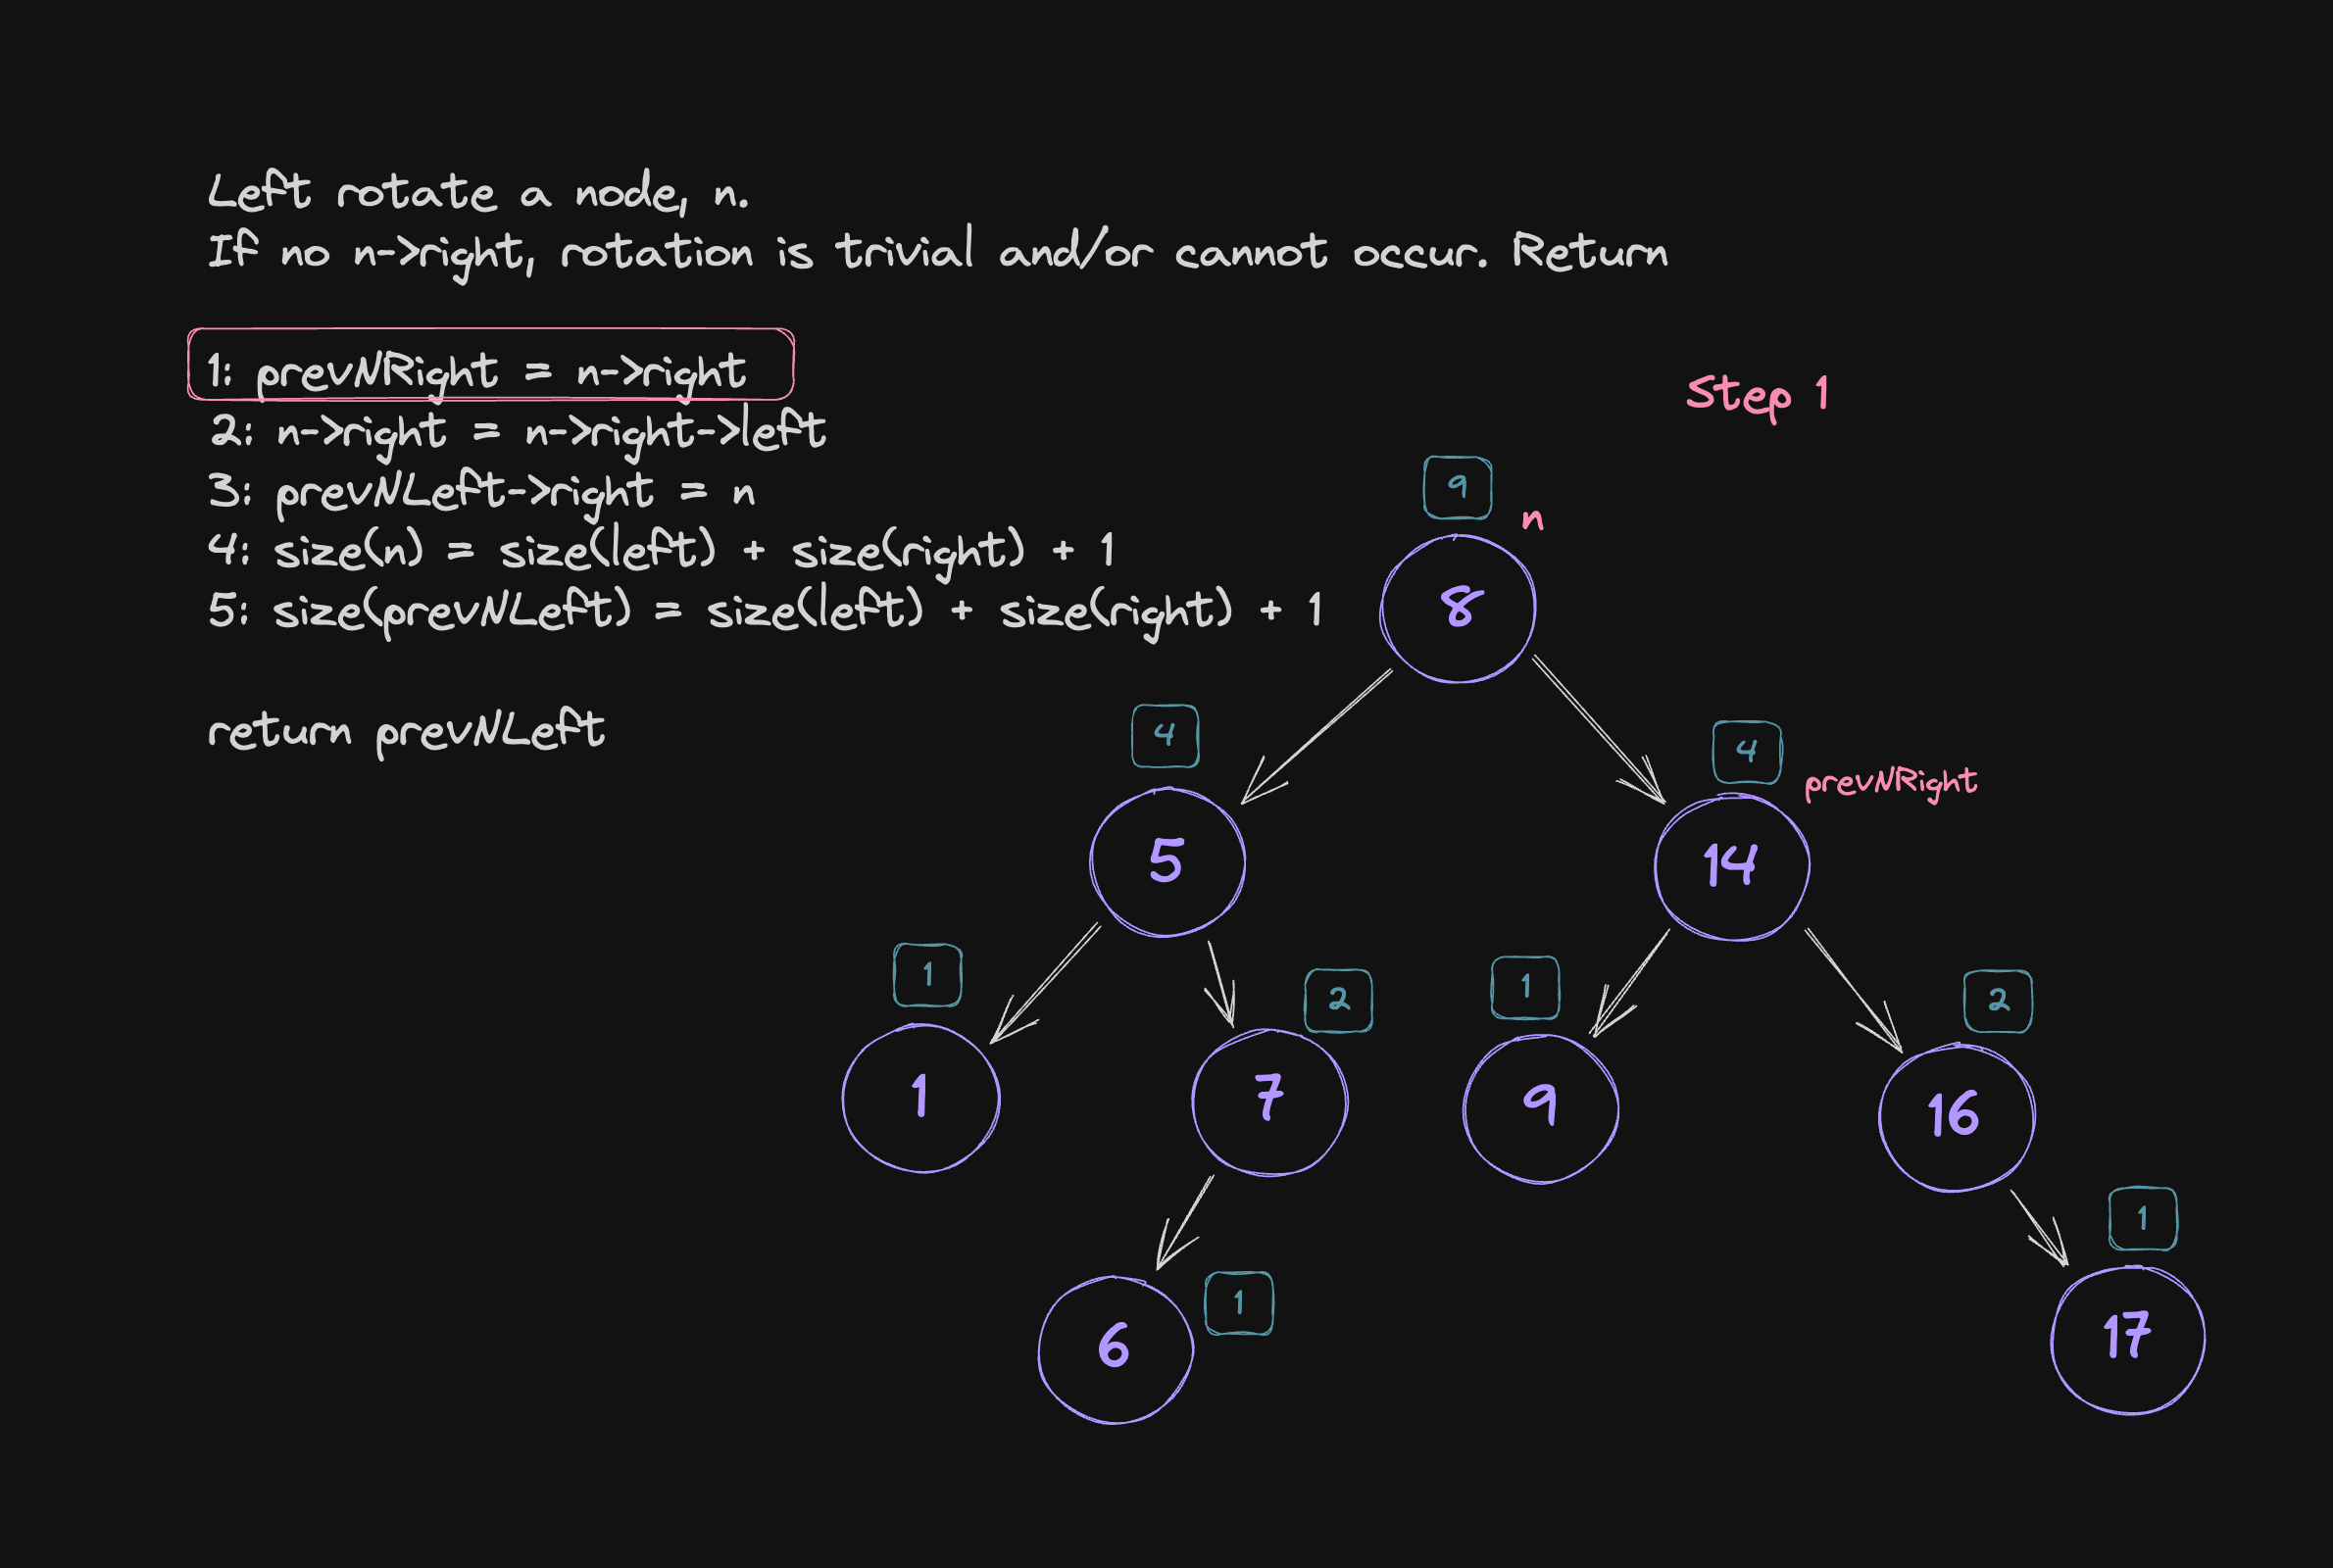
\includegraphics[scale=0.3]{left_rotations/lr1.png}         
           \newline
           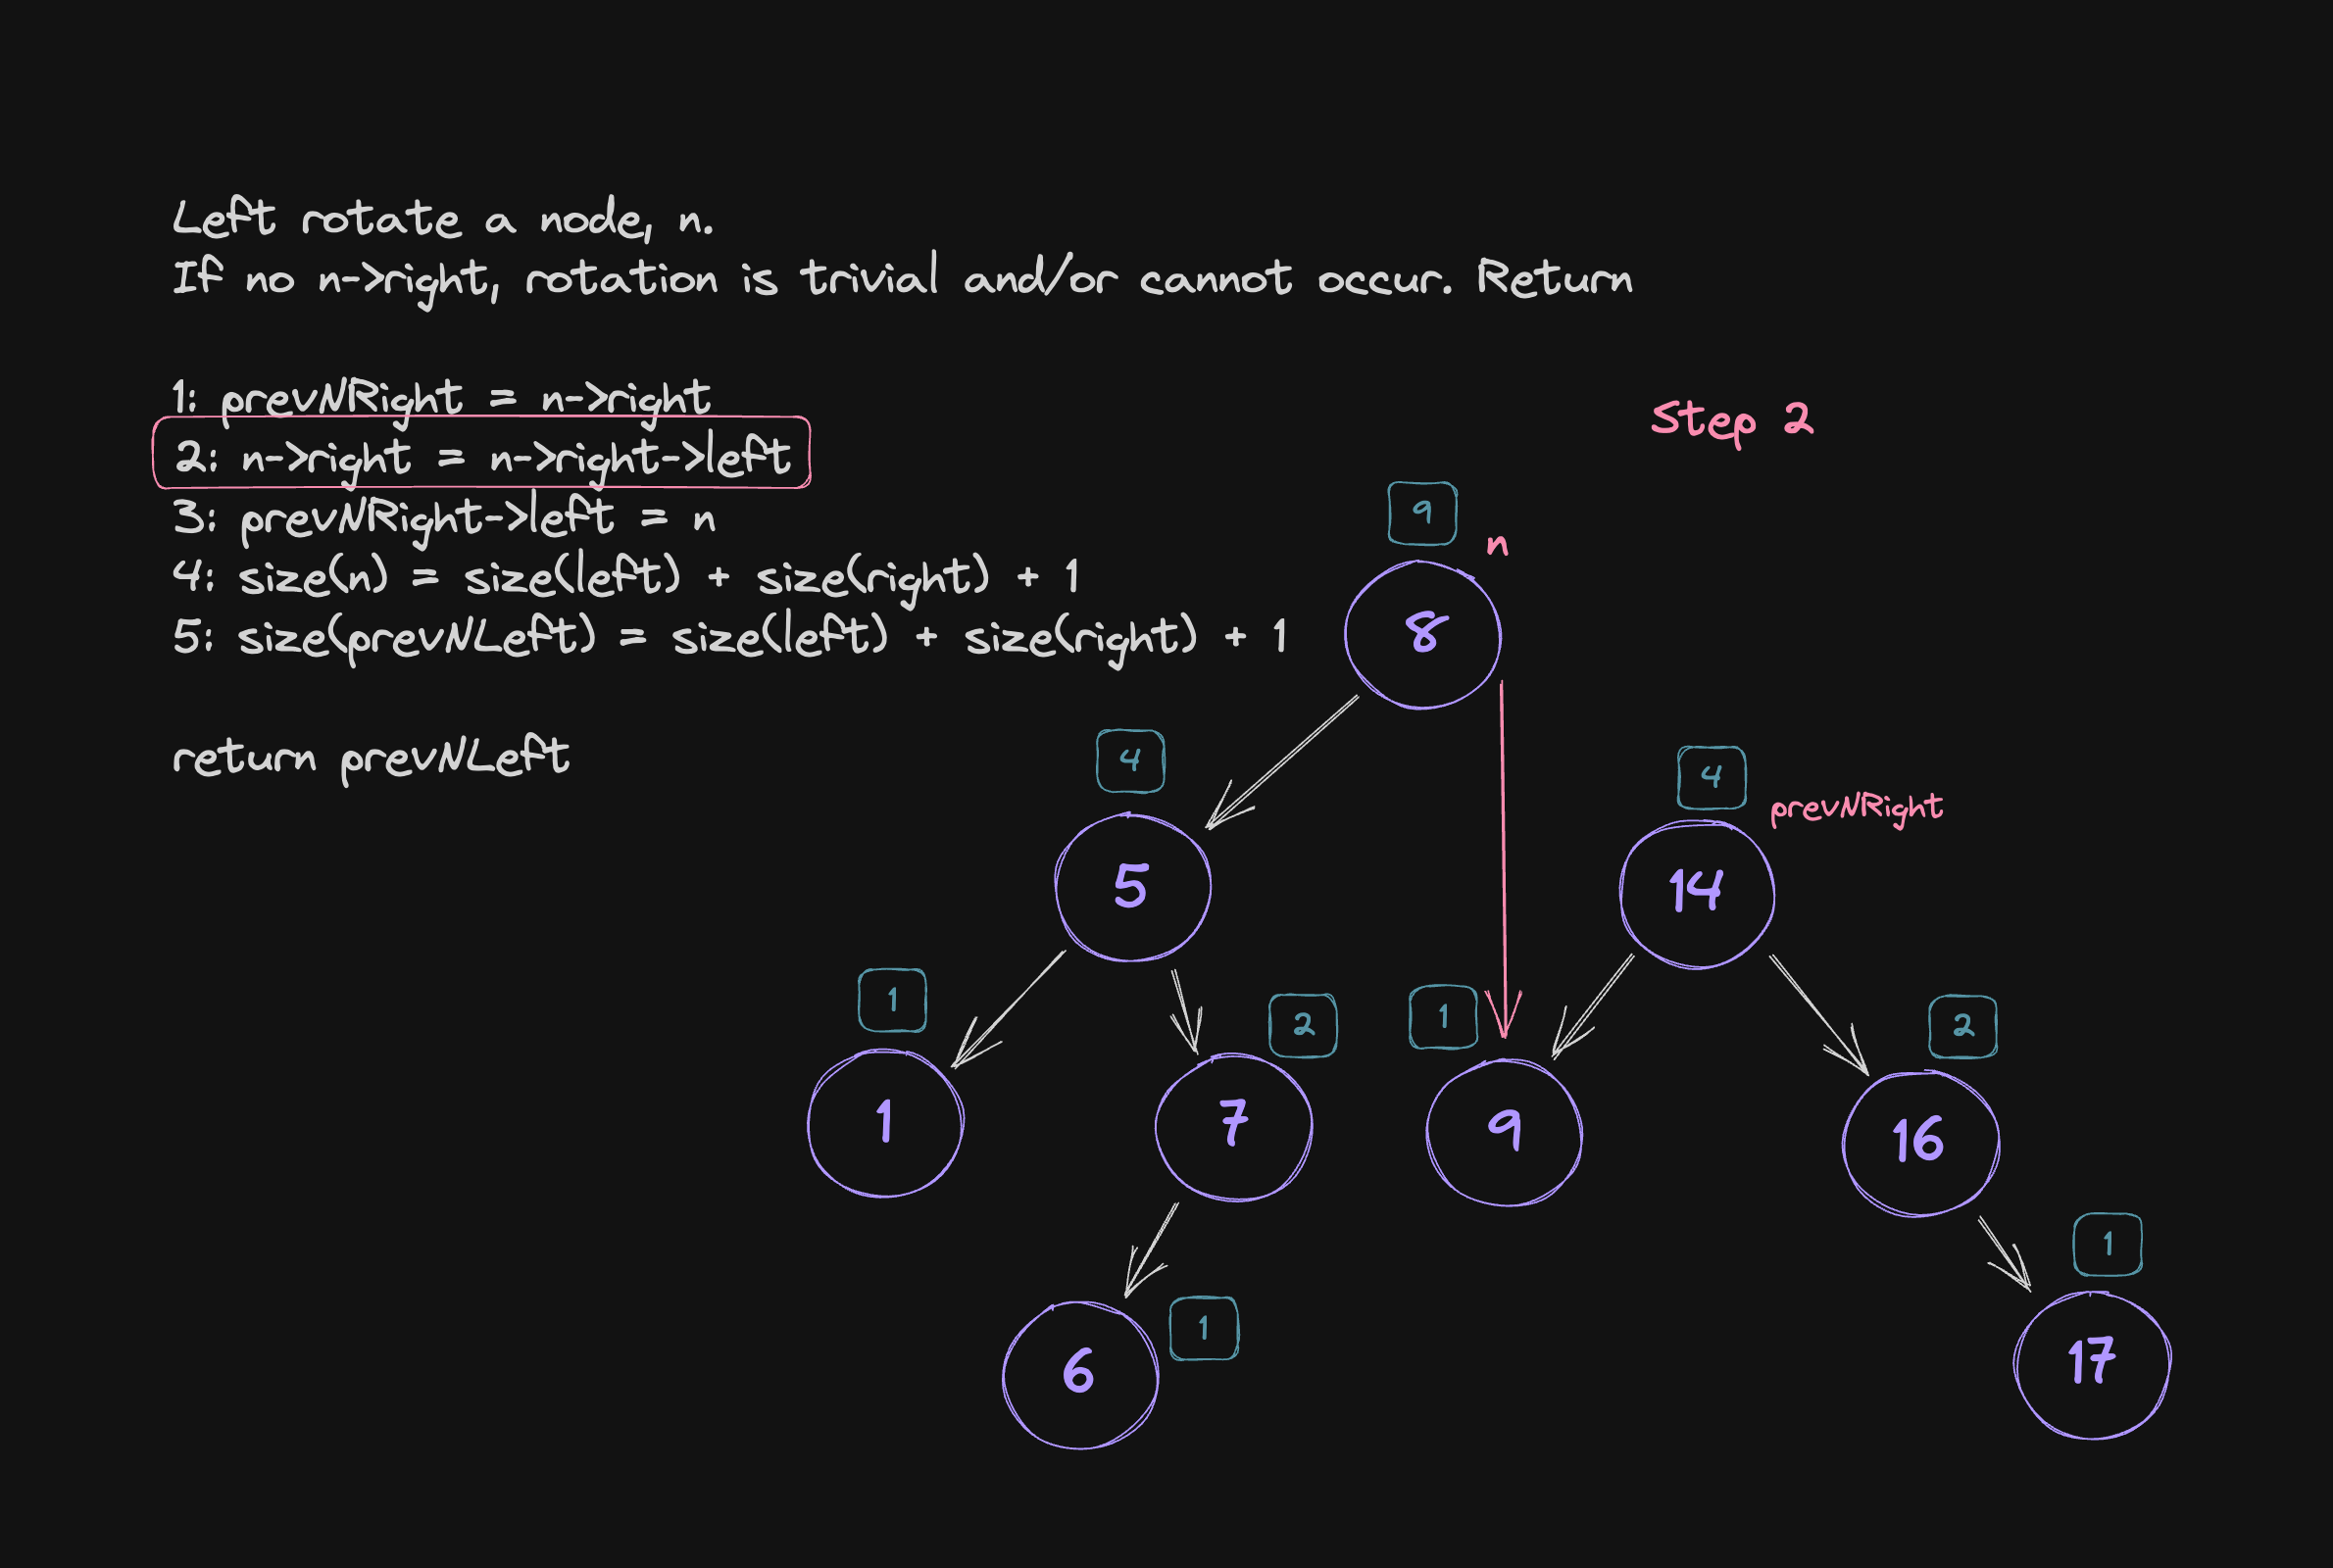
\includegraphics[scale=0.3]{left_rotations/lr2.png}         
           \newline
           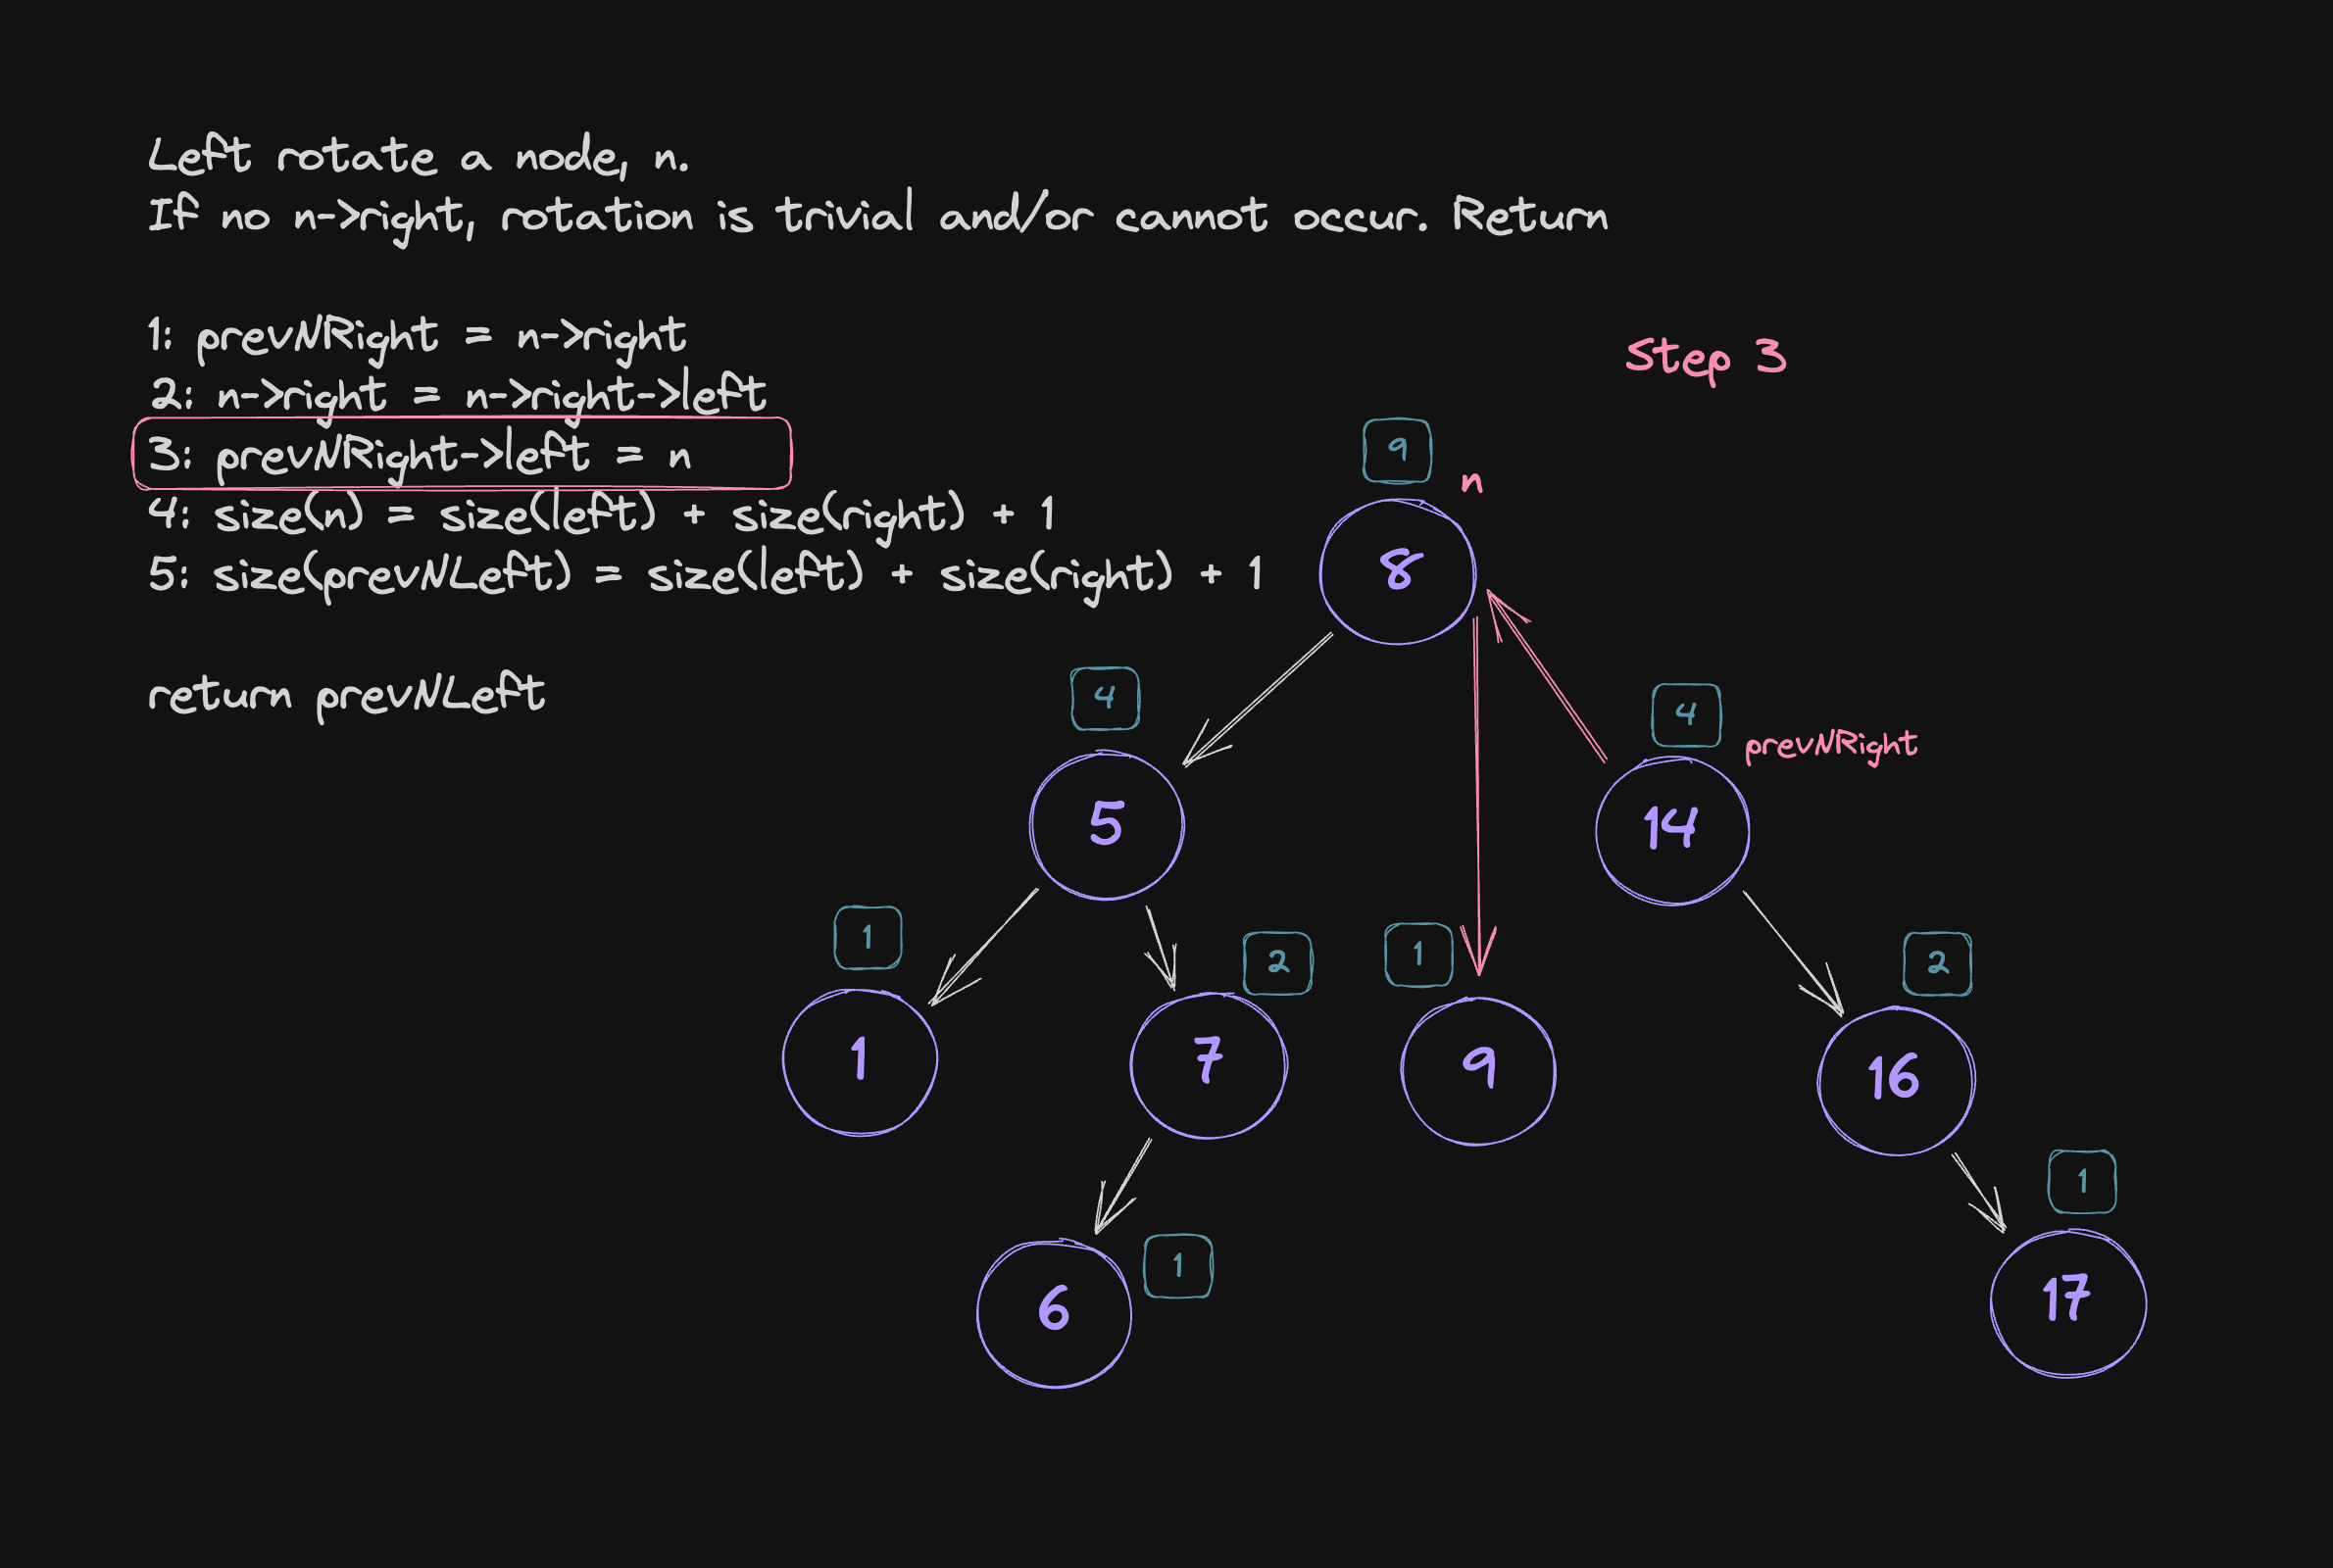
\includegraphics[scale=0.3]{left_rotations/lr3.png}         
           \newline
           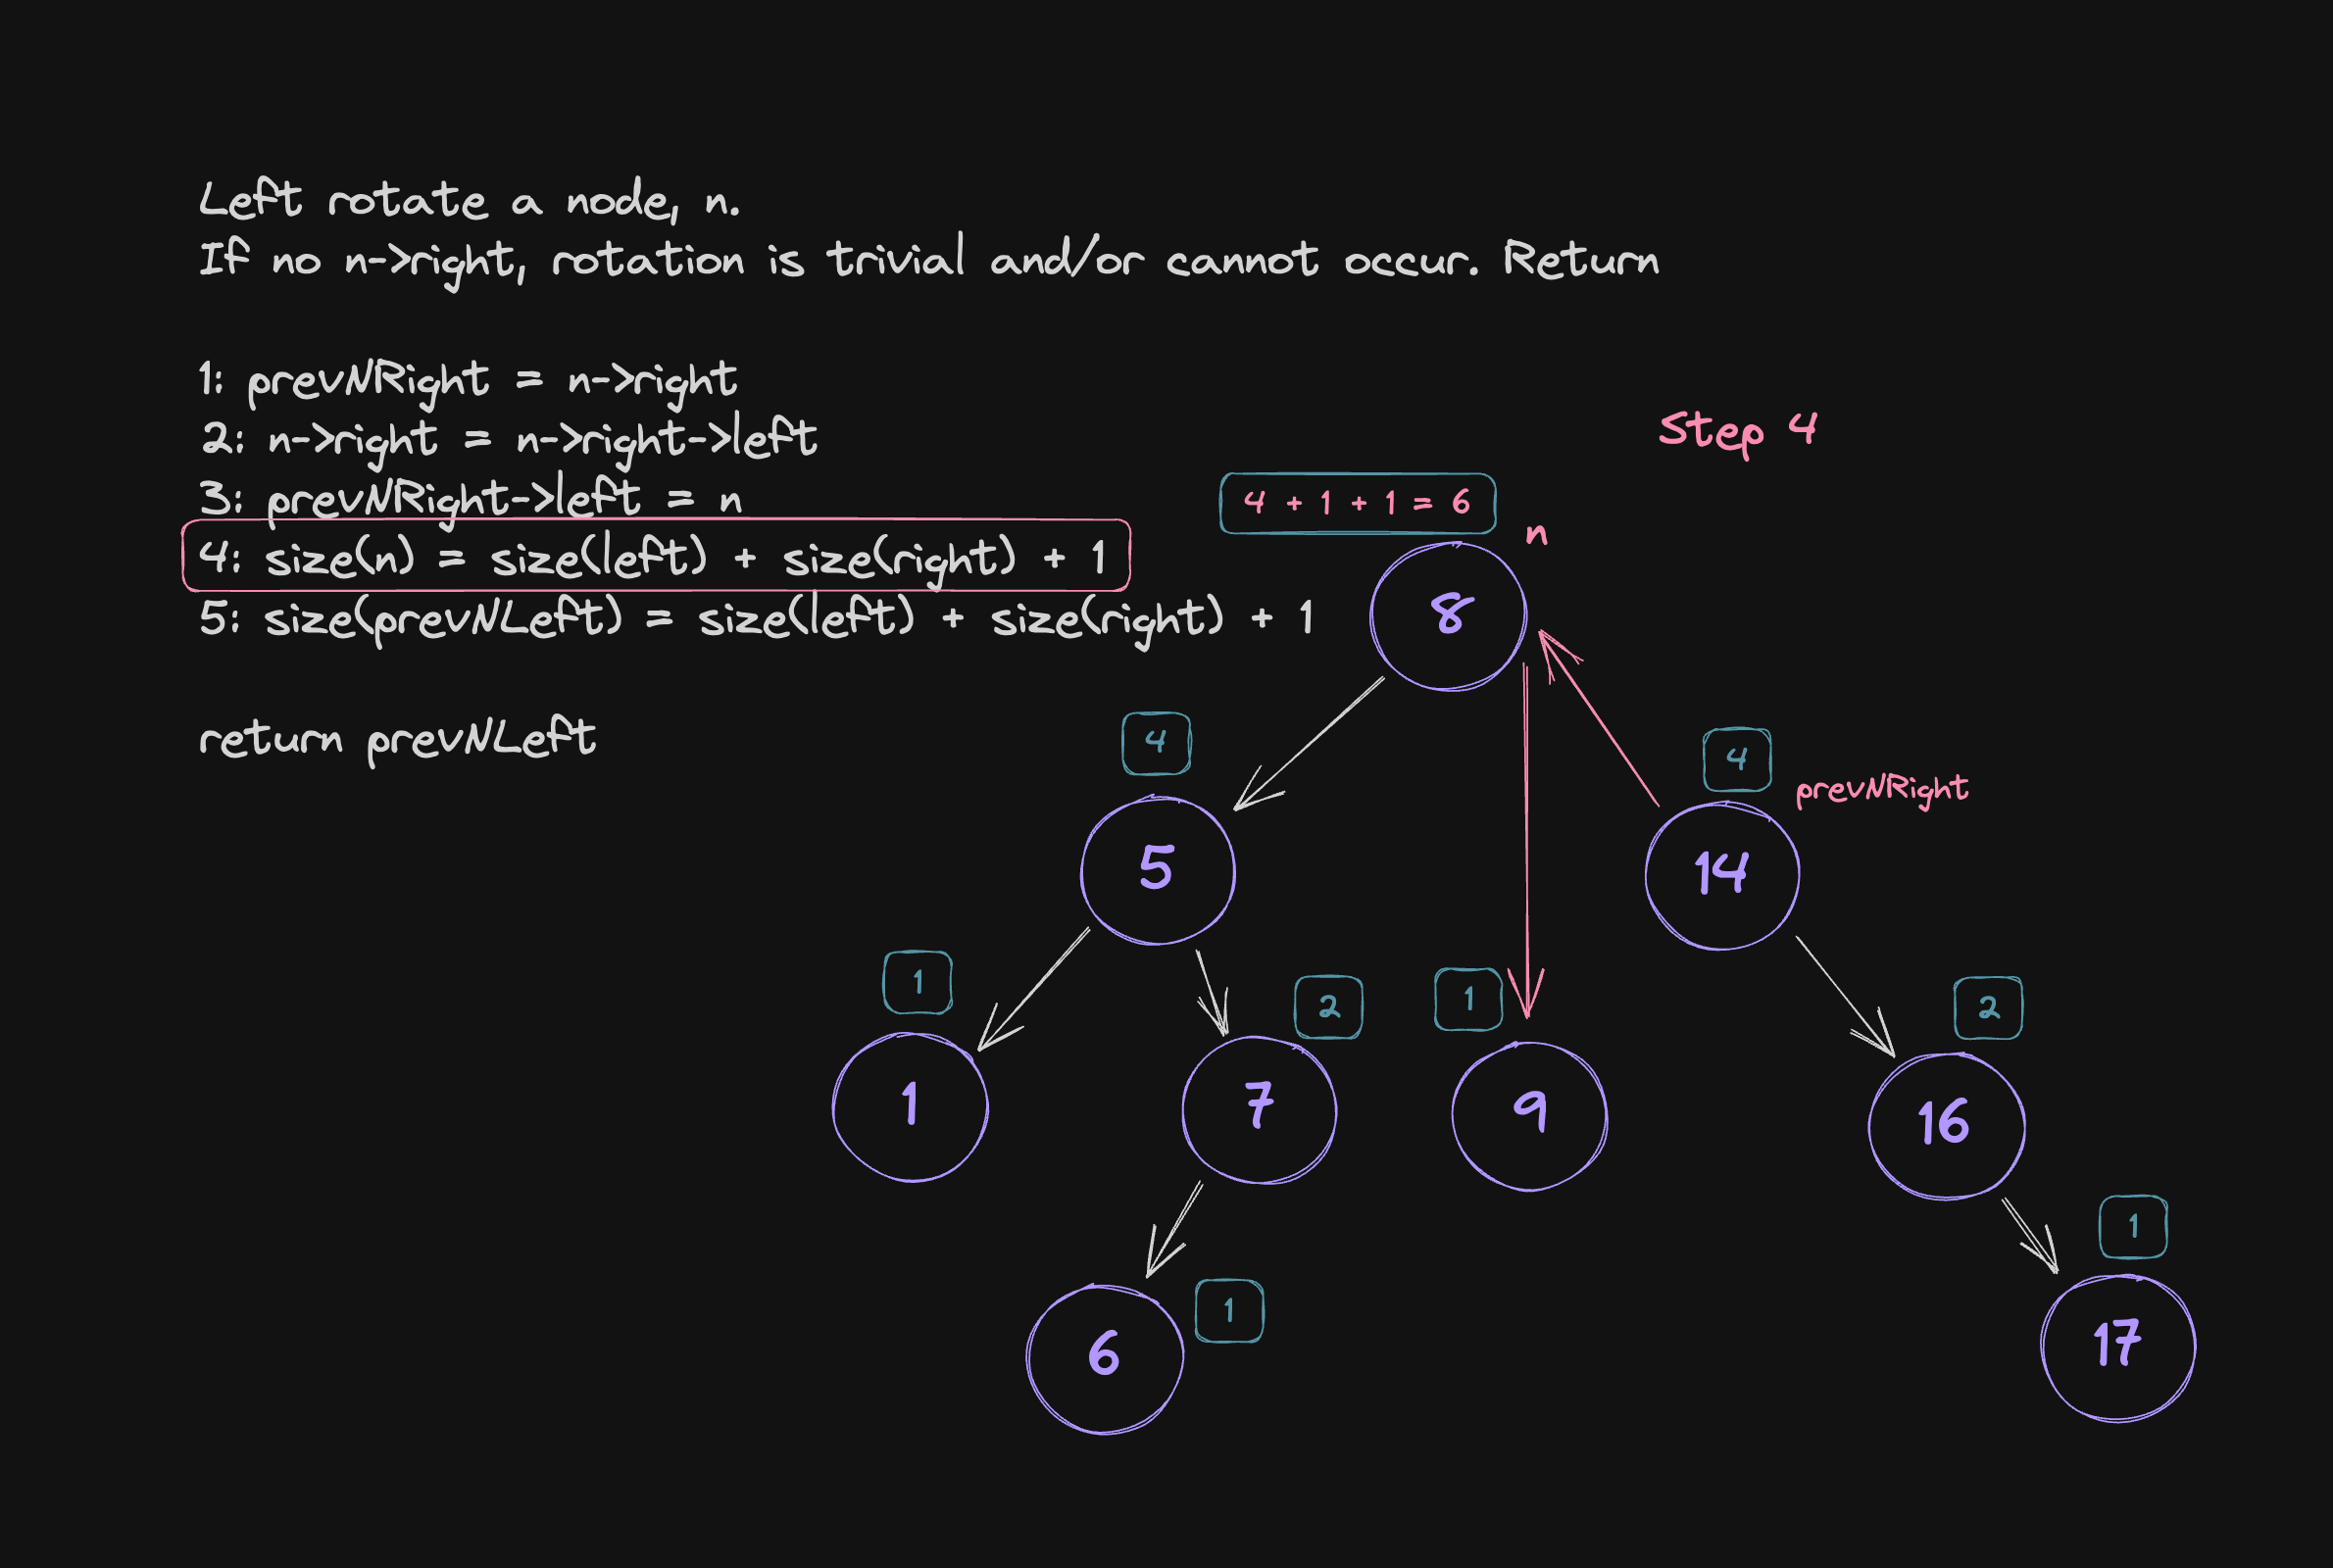
\includegraphics[scale=0.3]{left_rotations/lr4.png}         
           \newline
           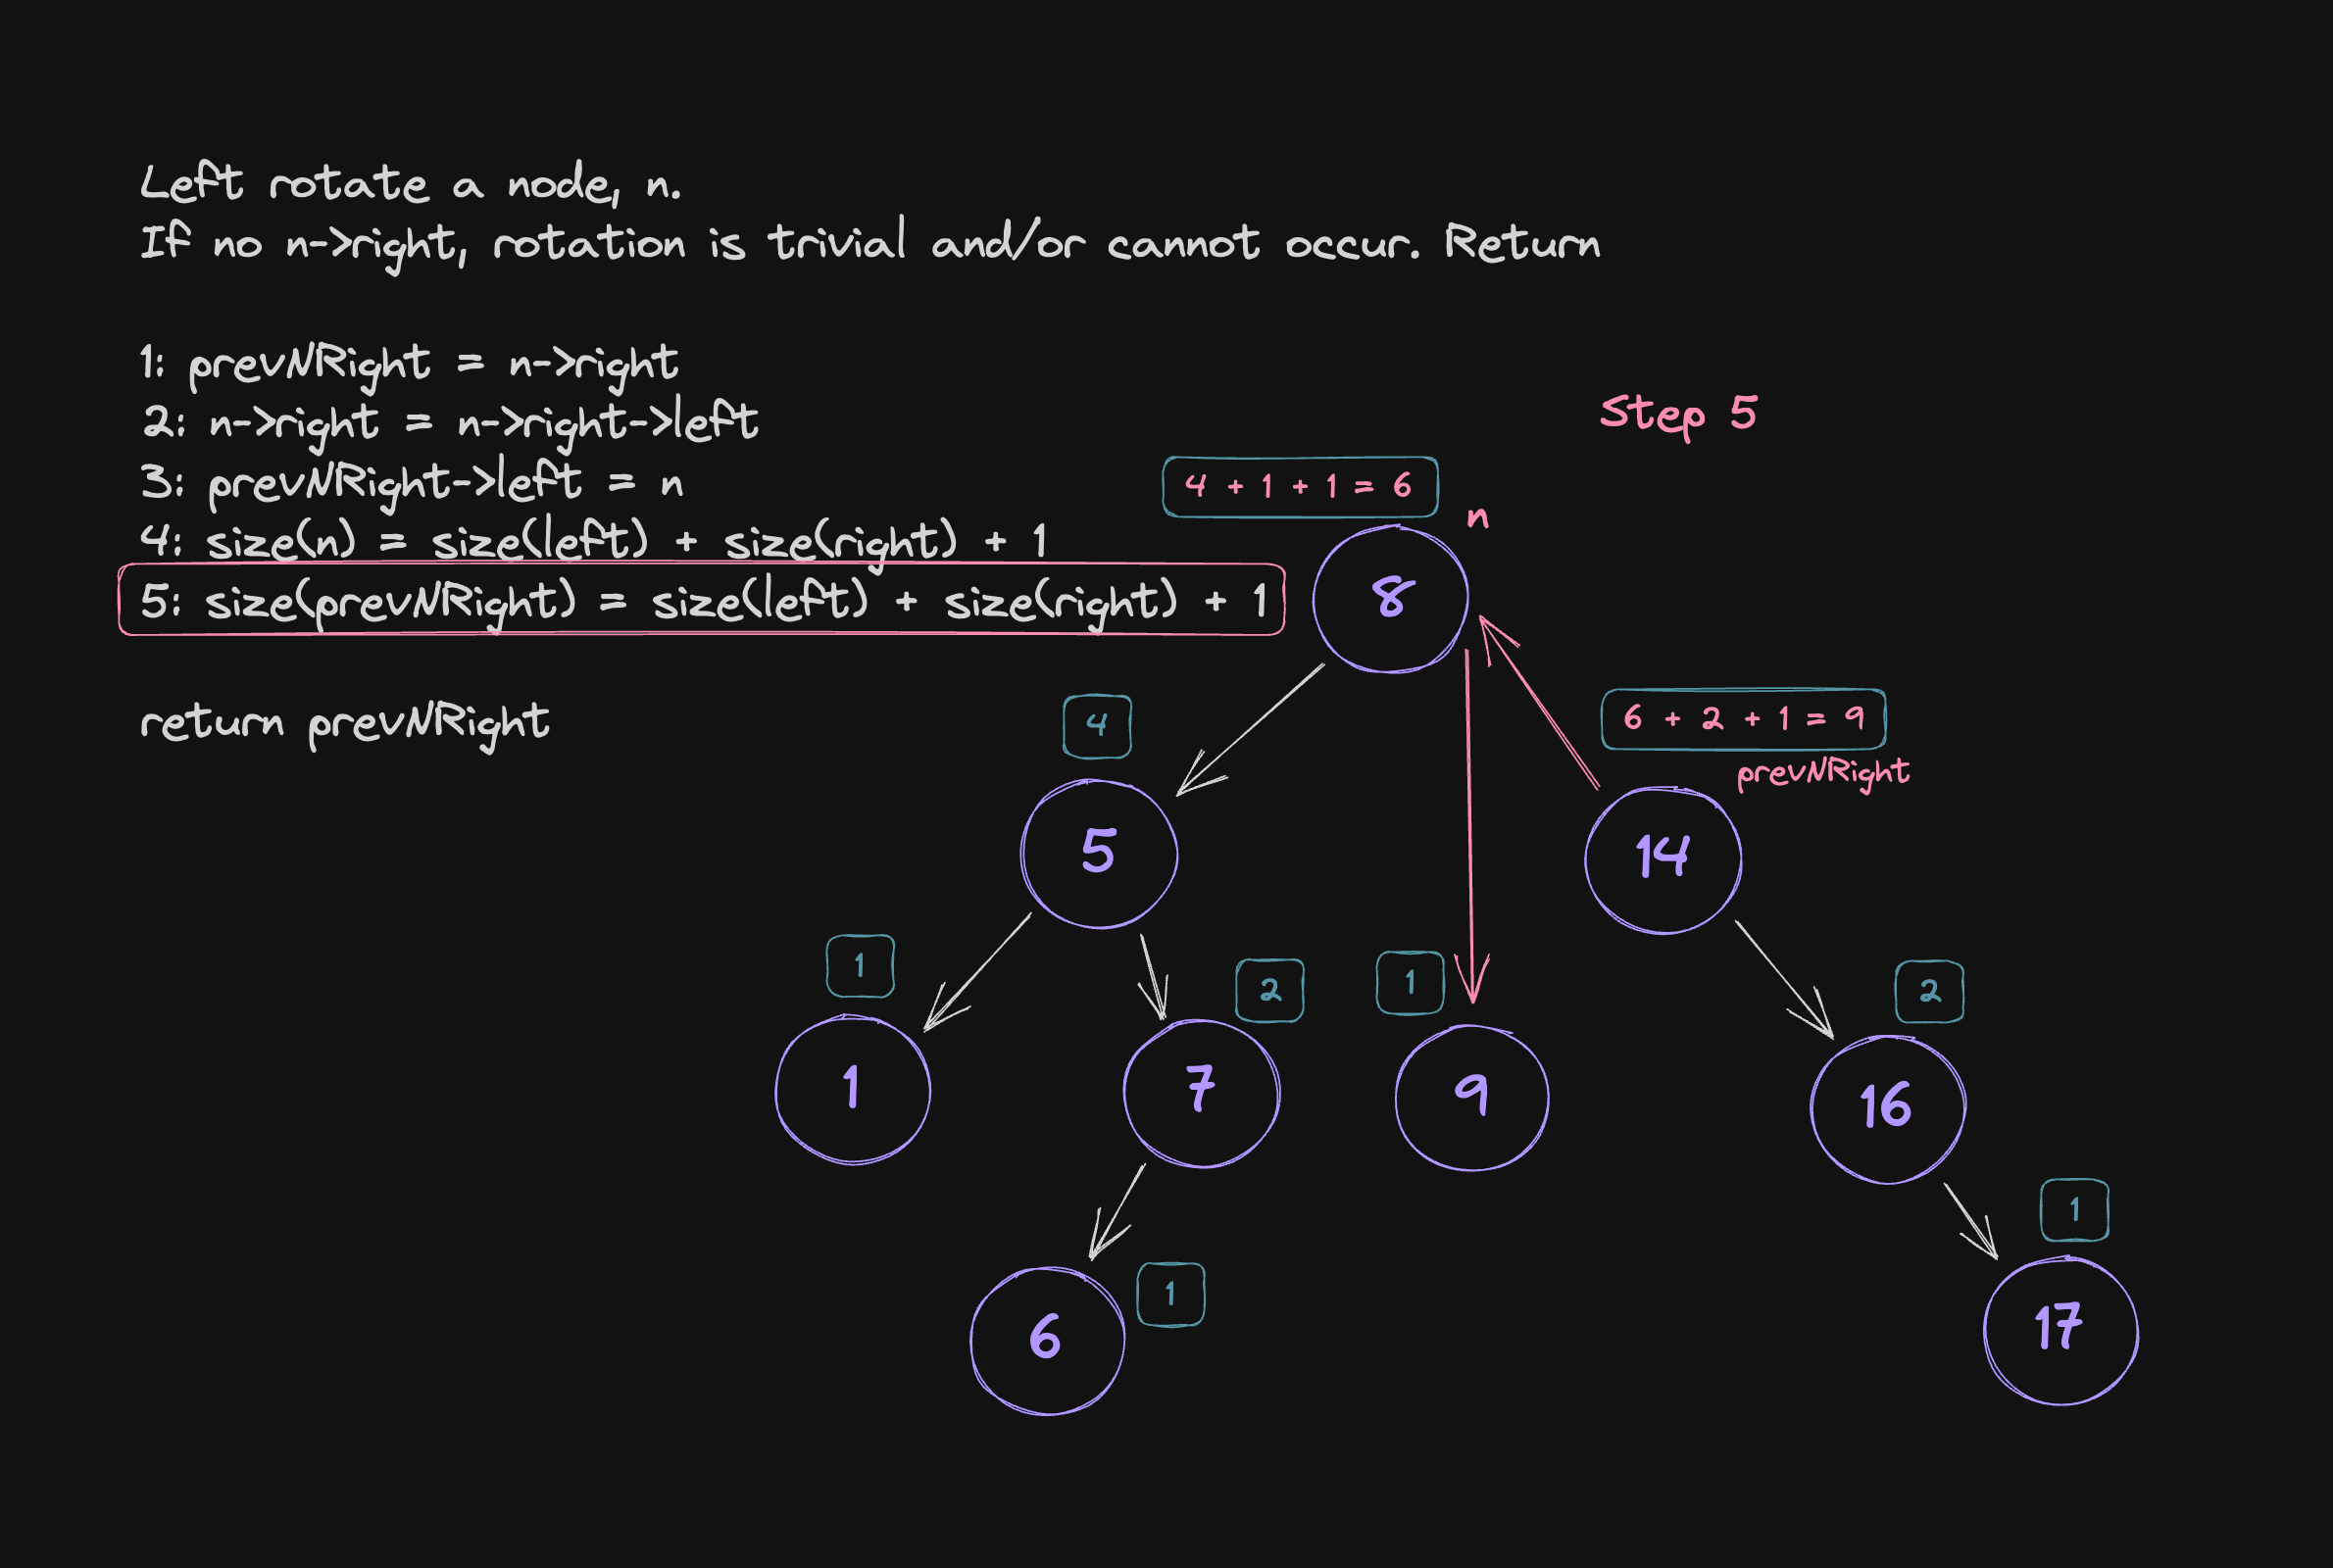
\includegraphics[scale=0.3]{left_rotations/lr5.png}         
           \newline
           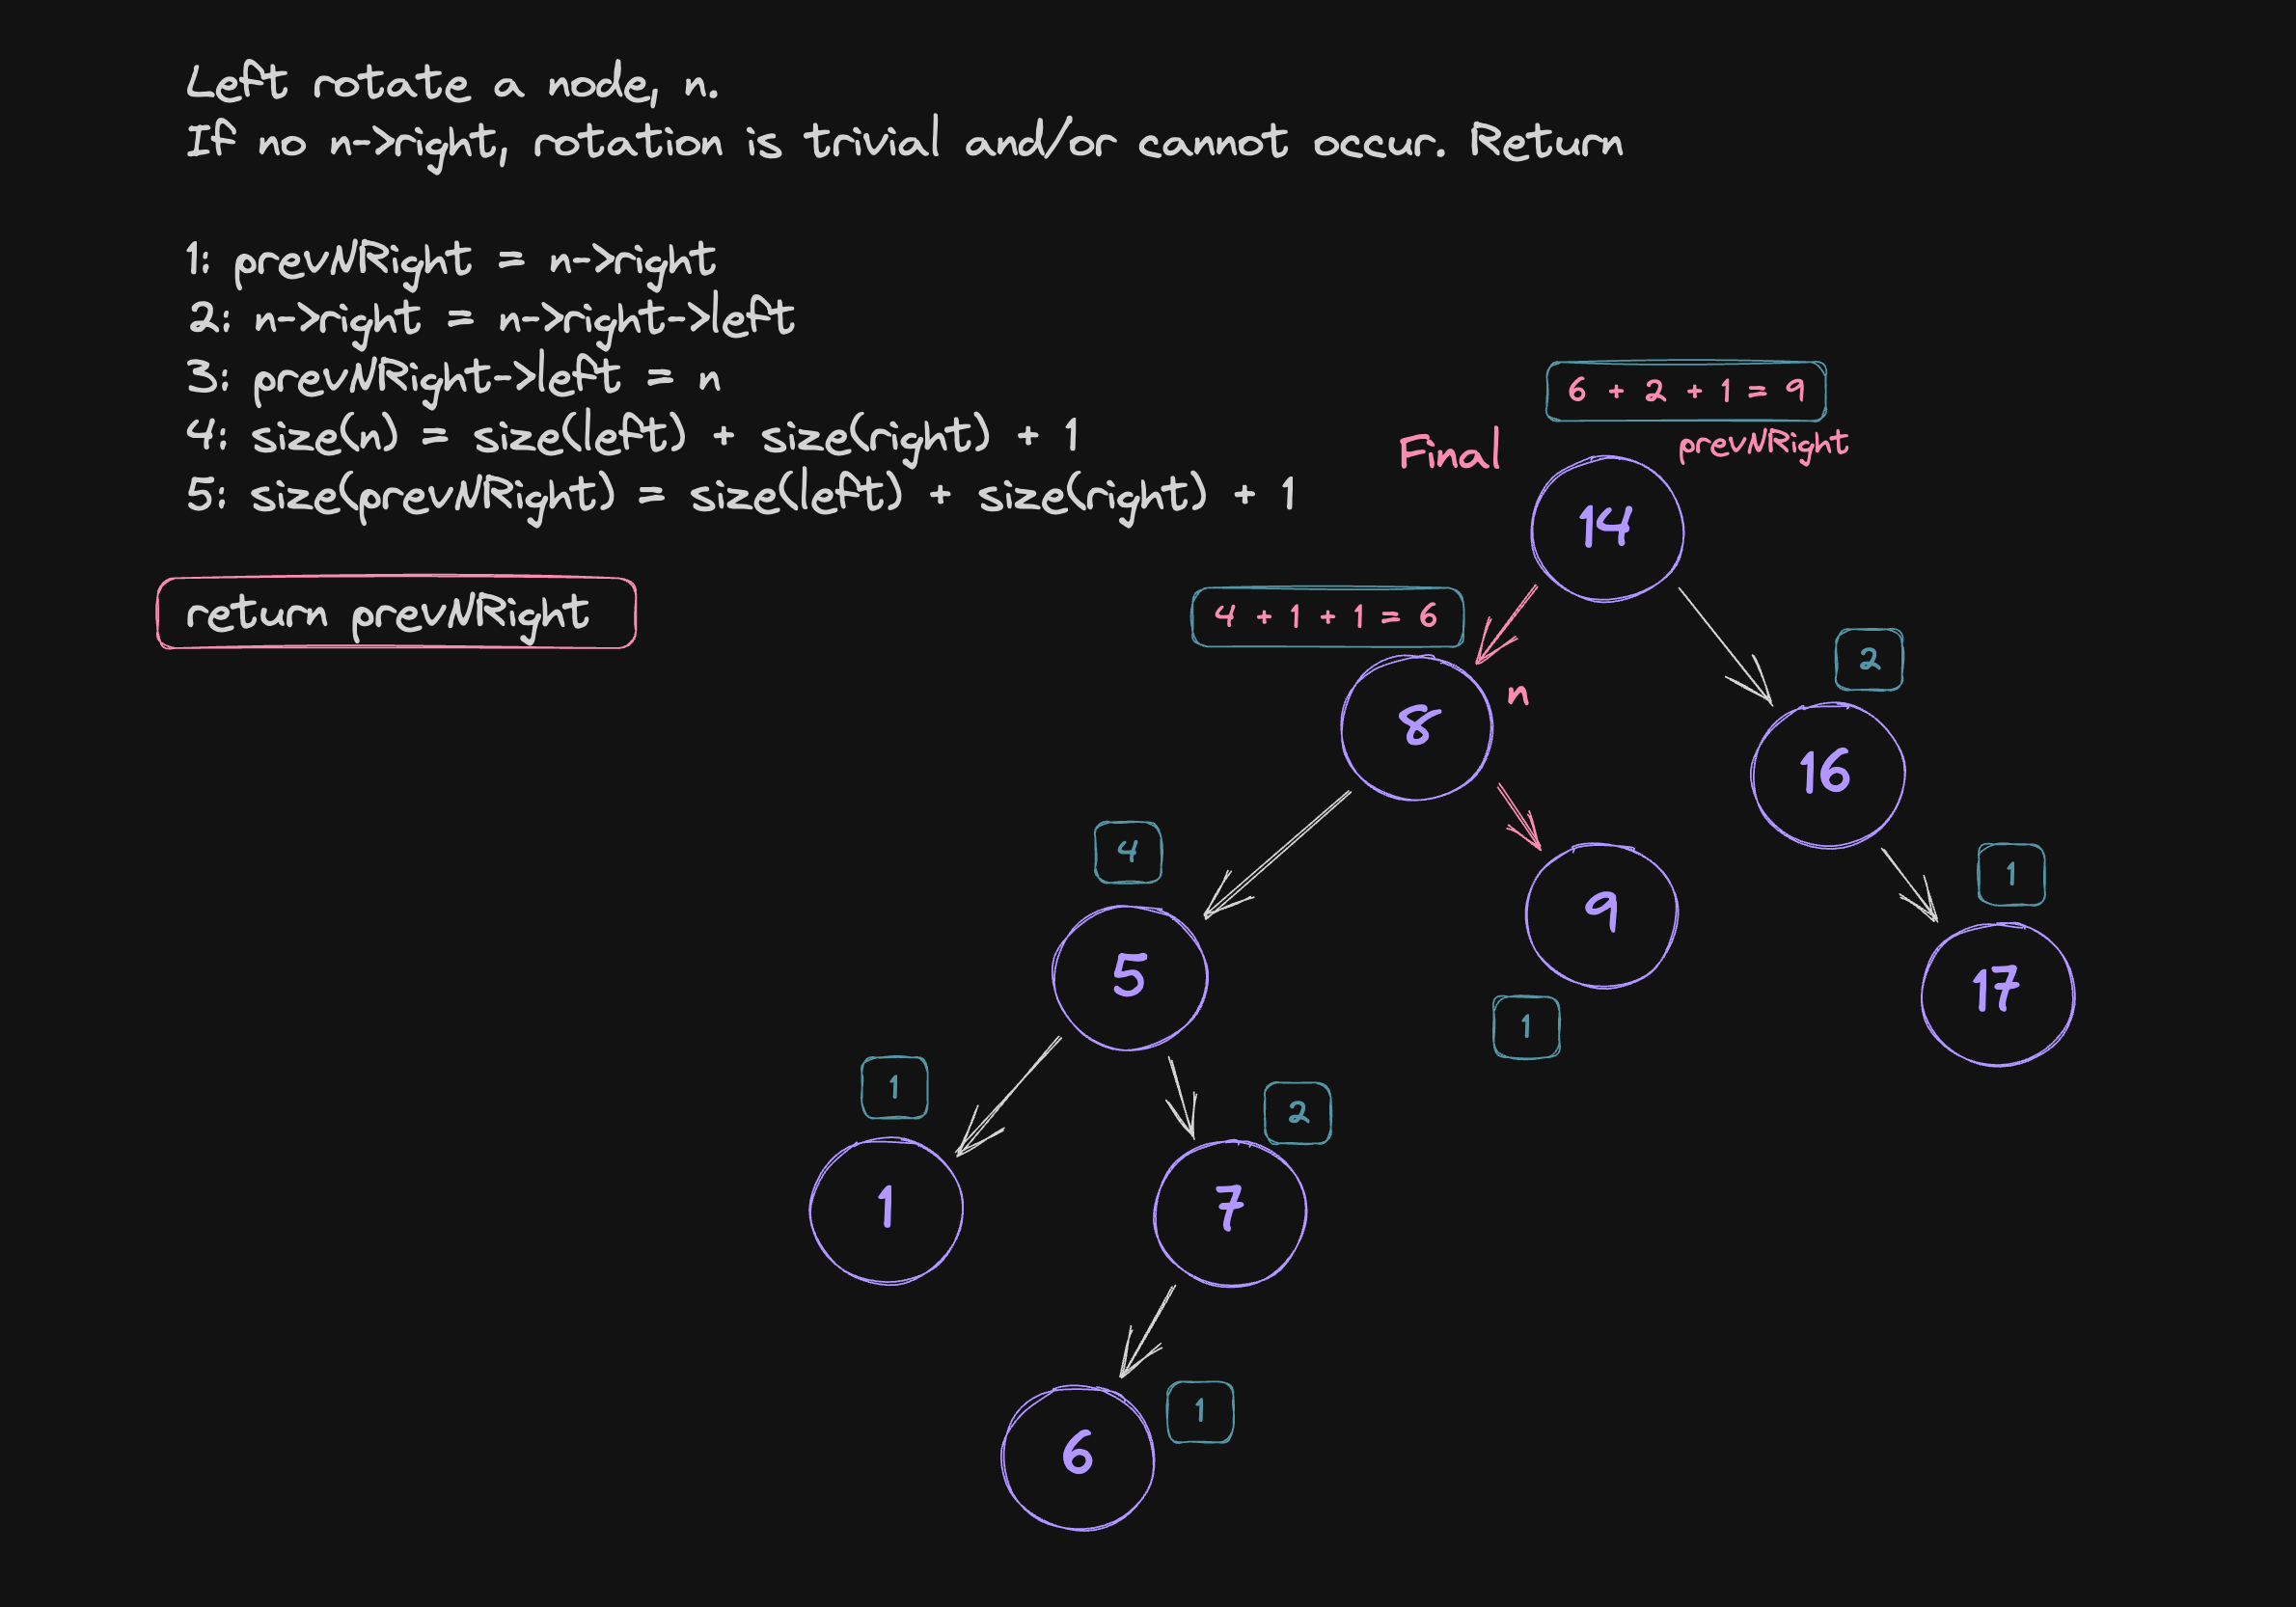
\includegraphics[scale=0.3]{left_rotations/lrf.png}         
           \newline
            \newline
            \textbf{Right rotation}: \newline \newline
           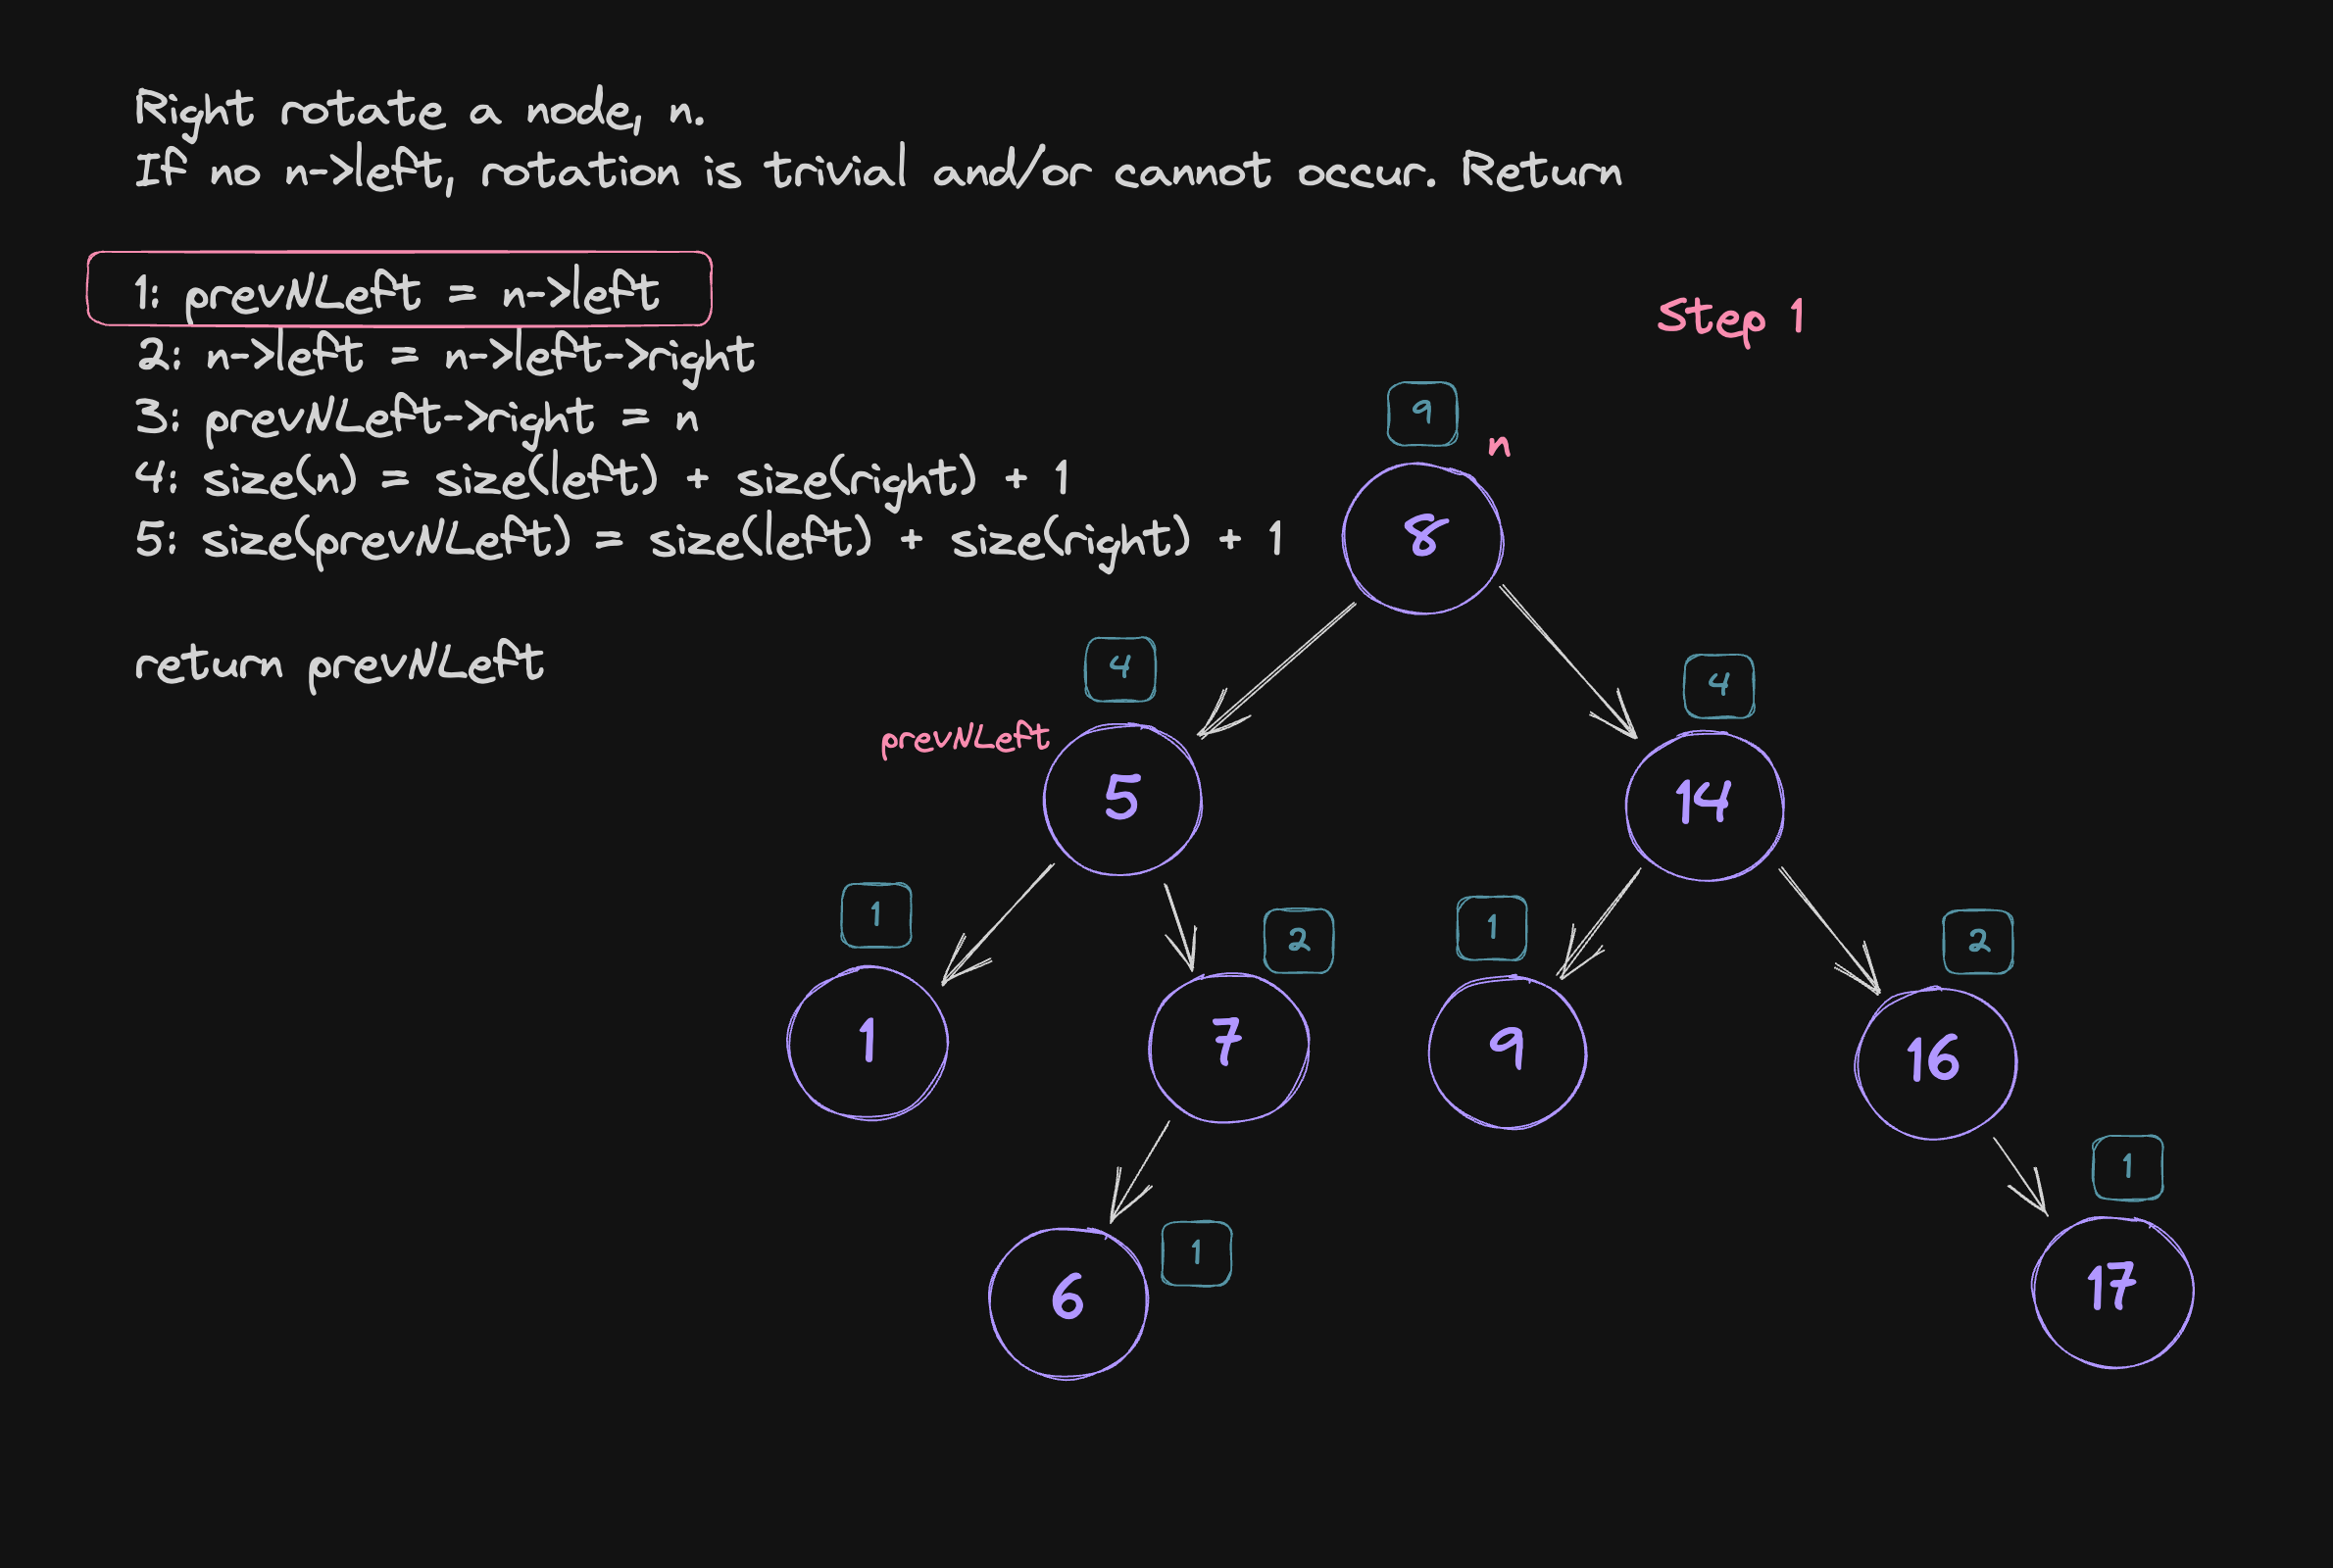
\includegraphics[scale=0.3]{right_rotations/rr1.png}         
           \newline
           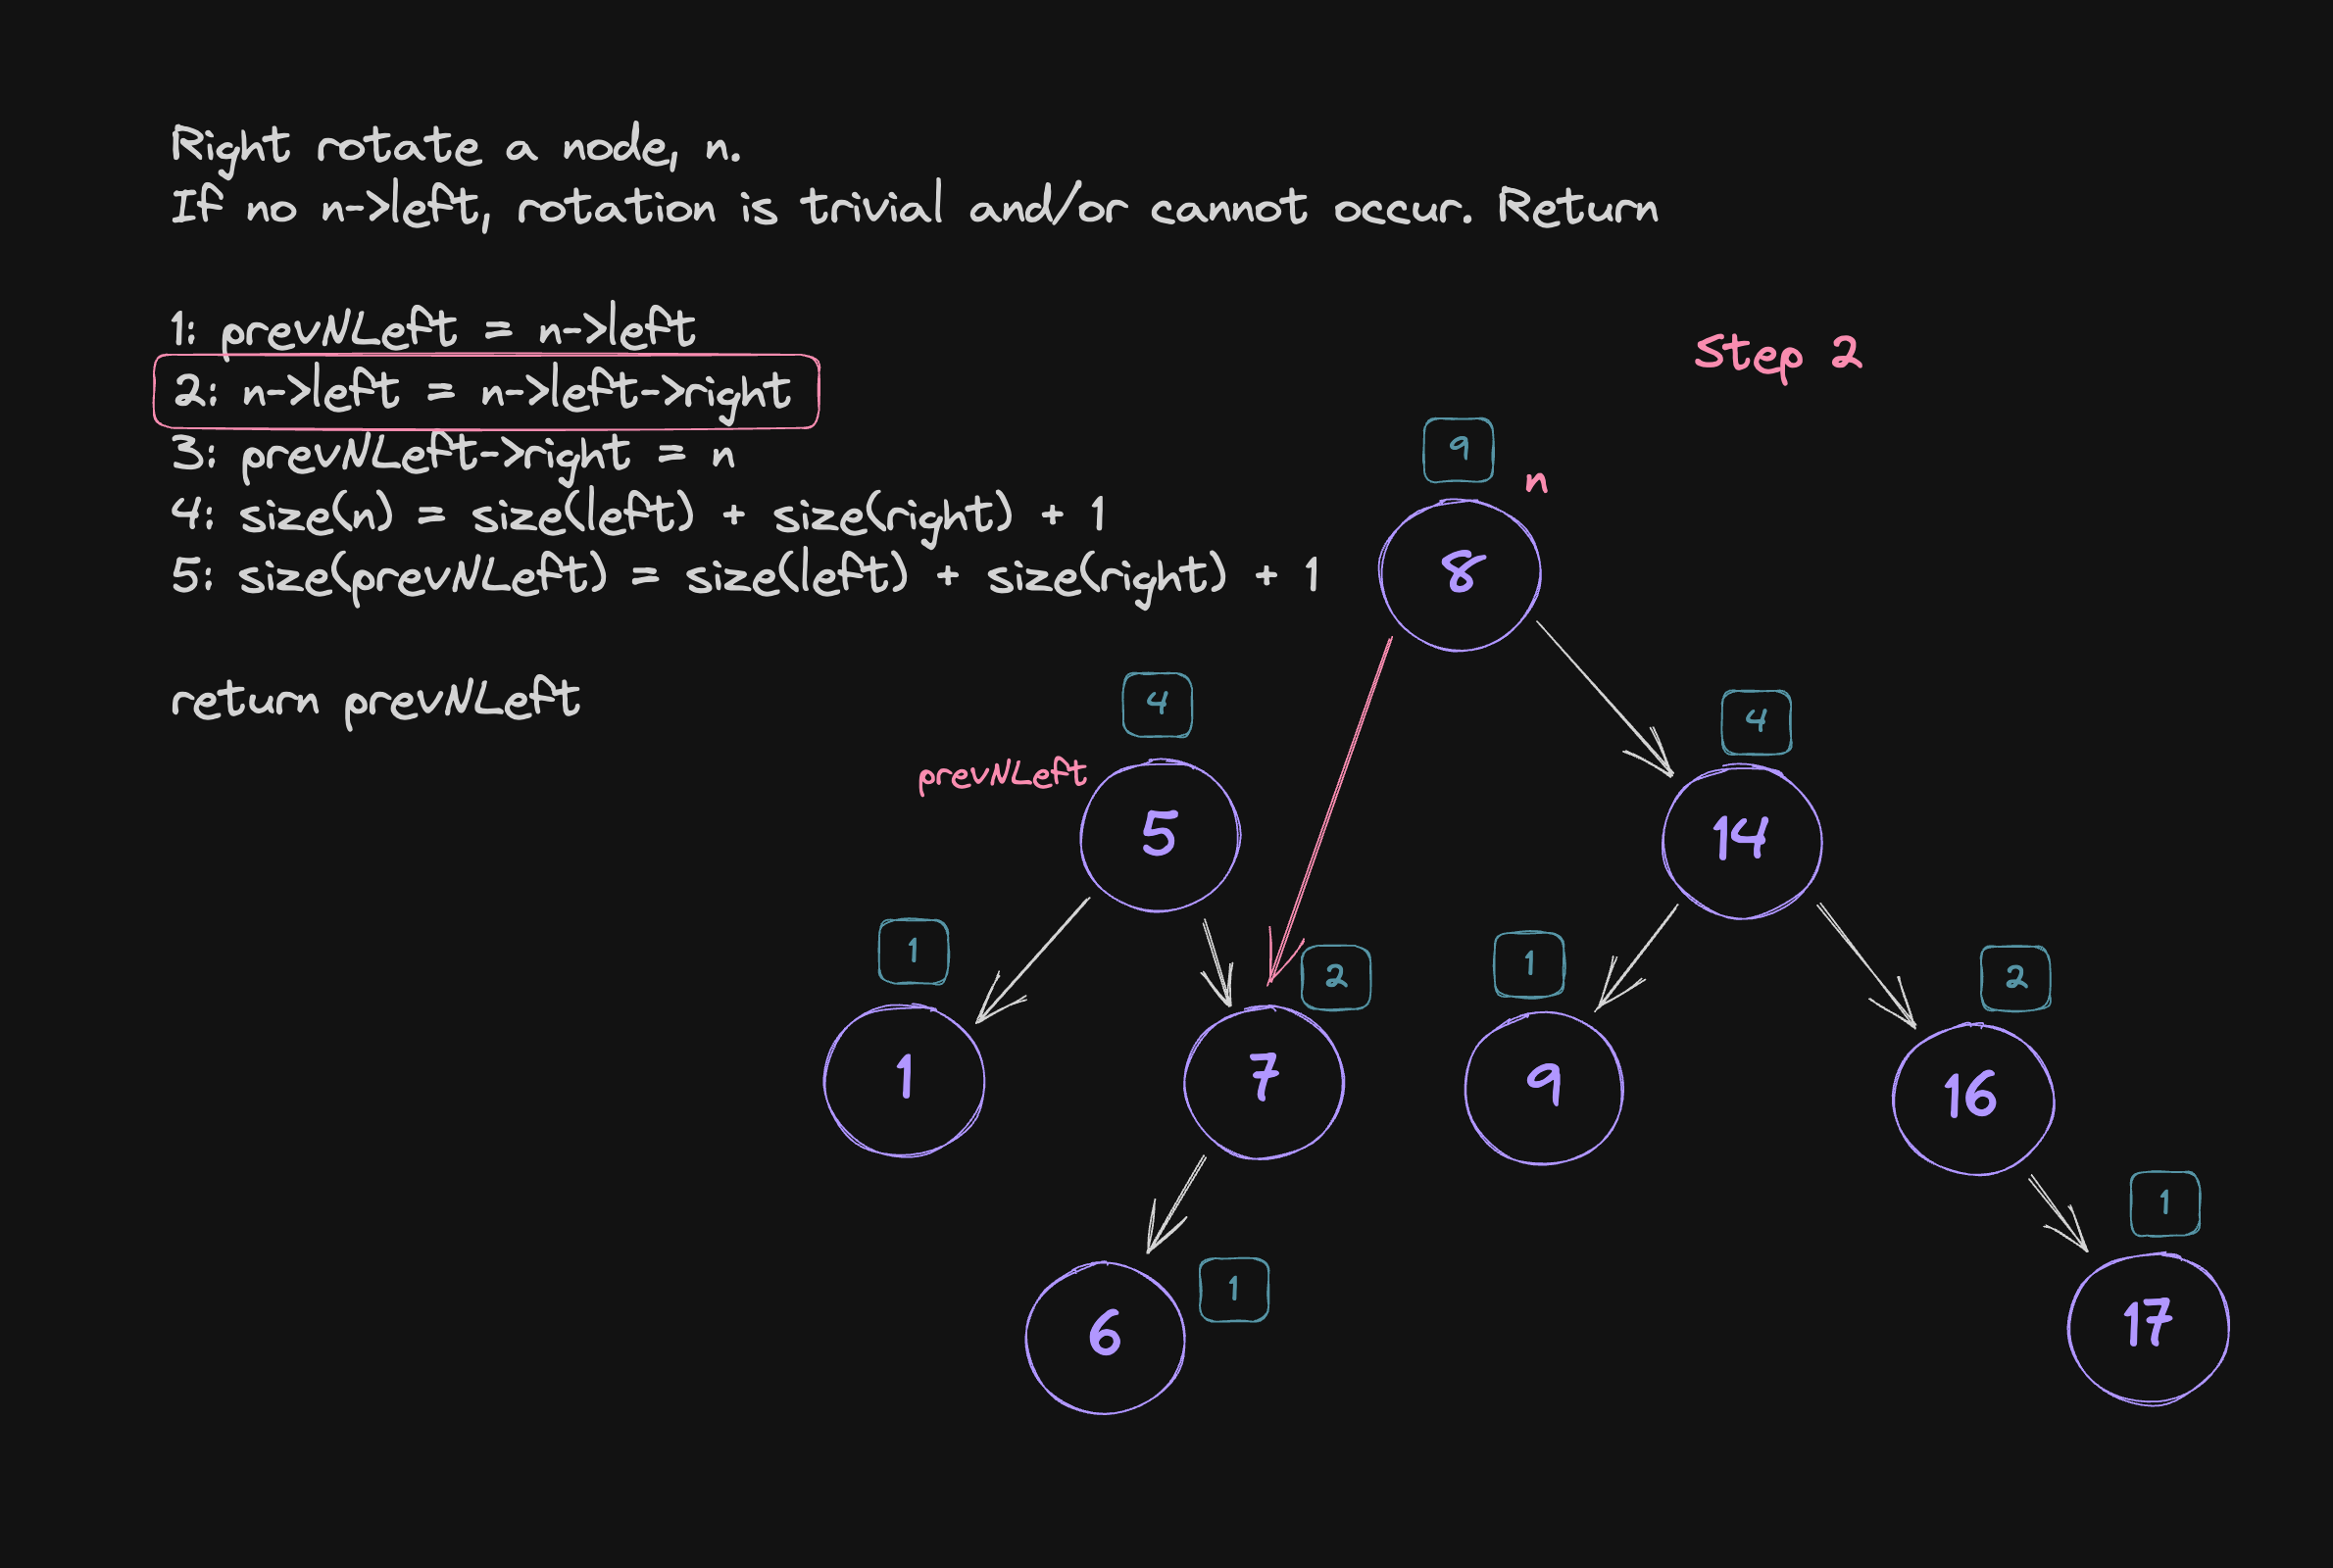
\includegraphics[scale=0.3]{right_rotations/rr2.png}         
           \newline
           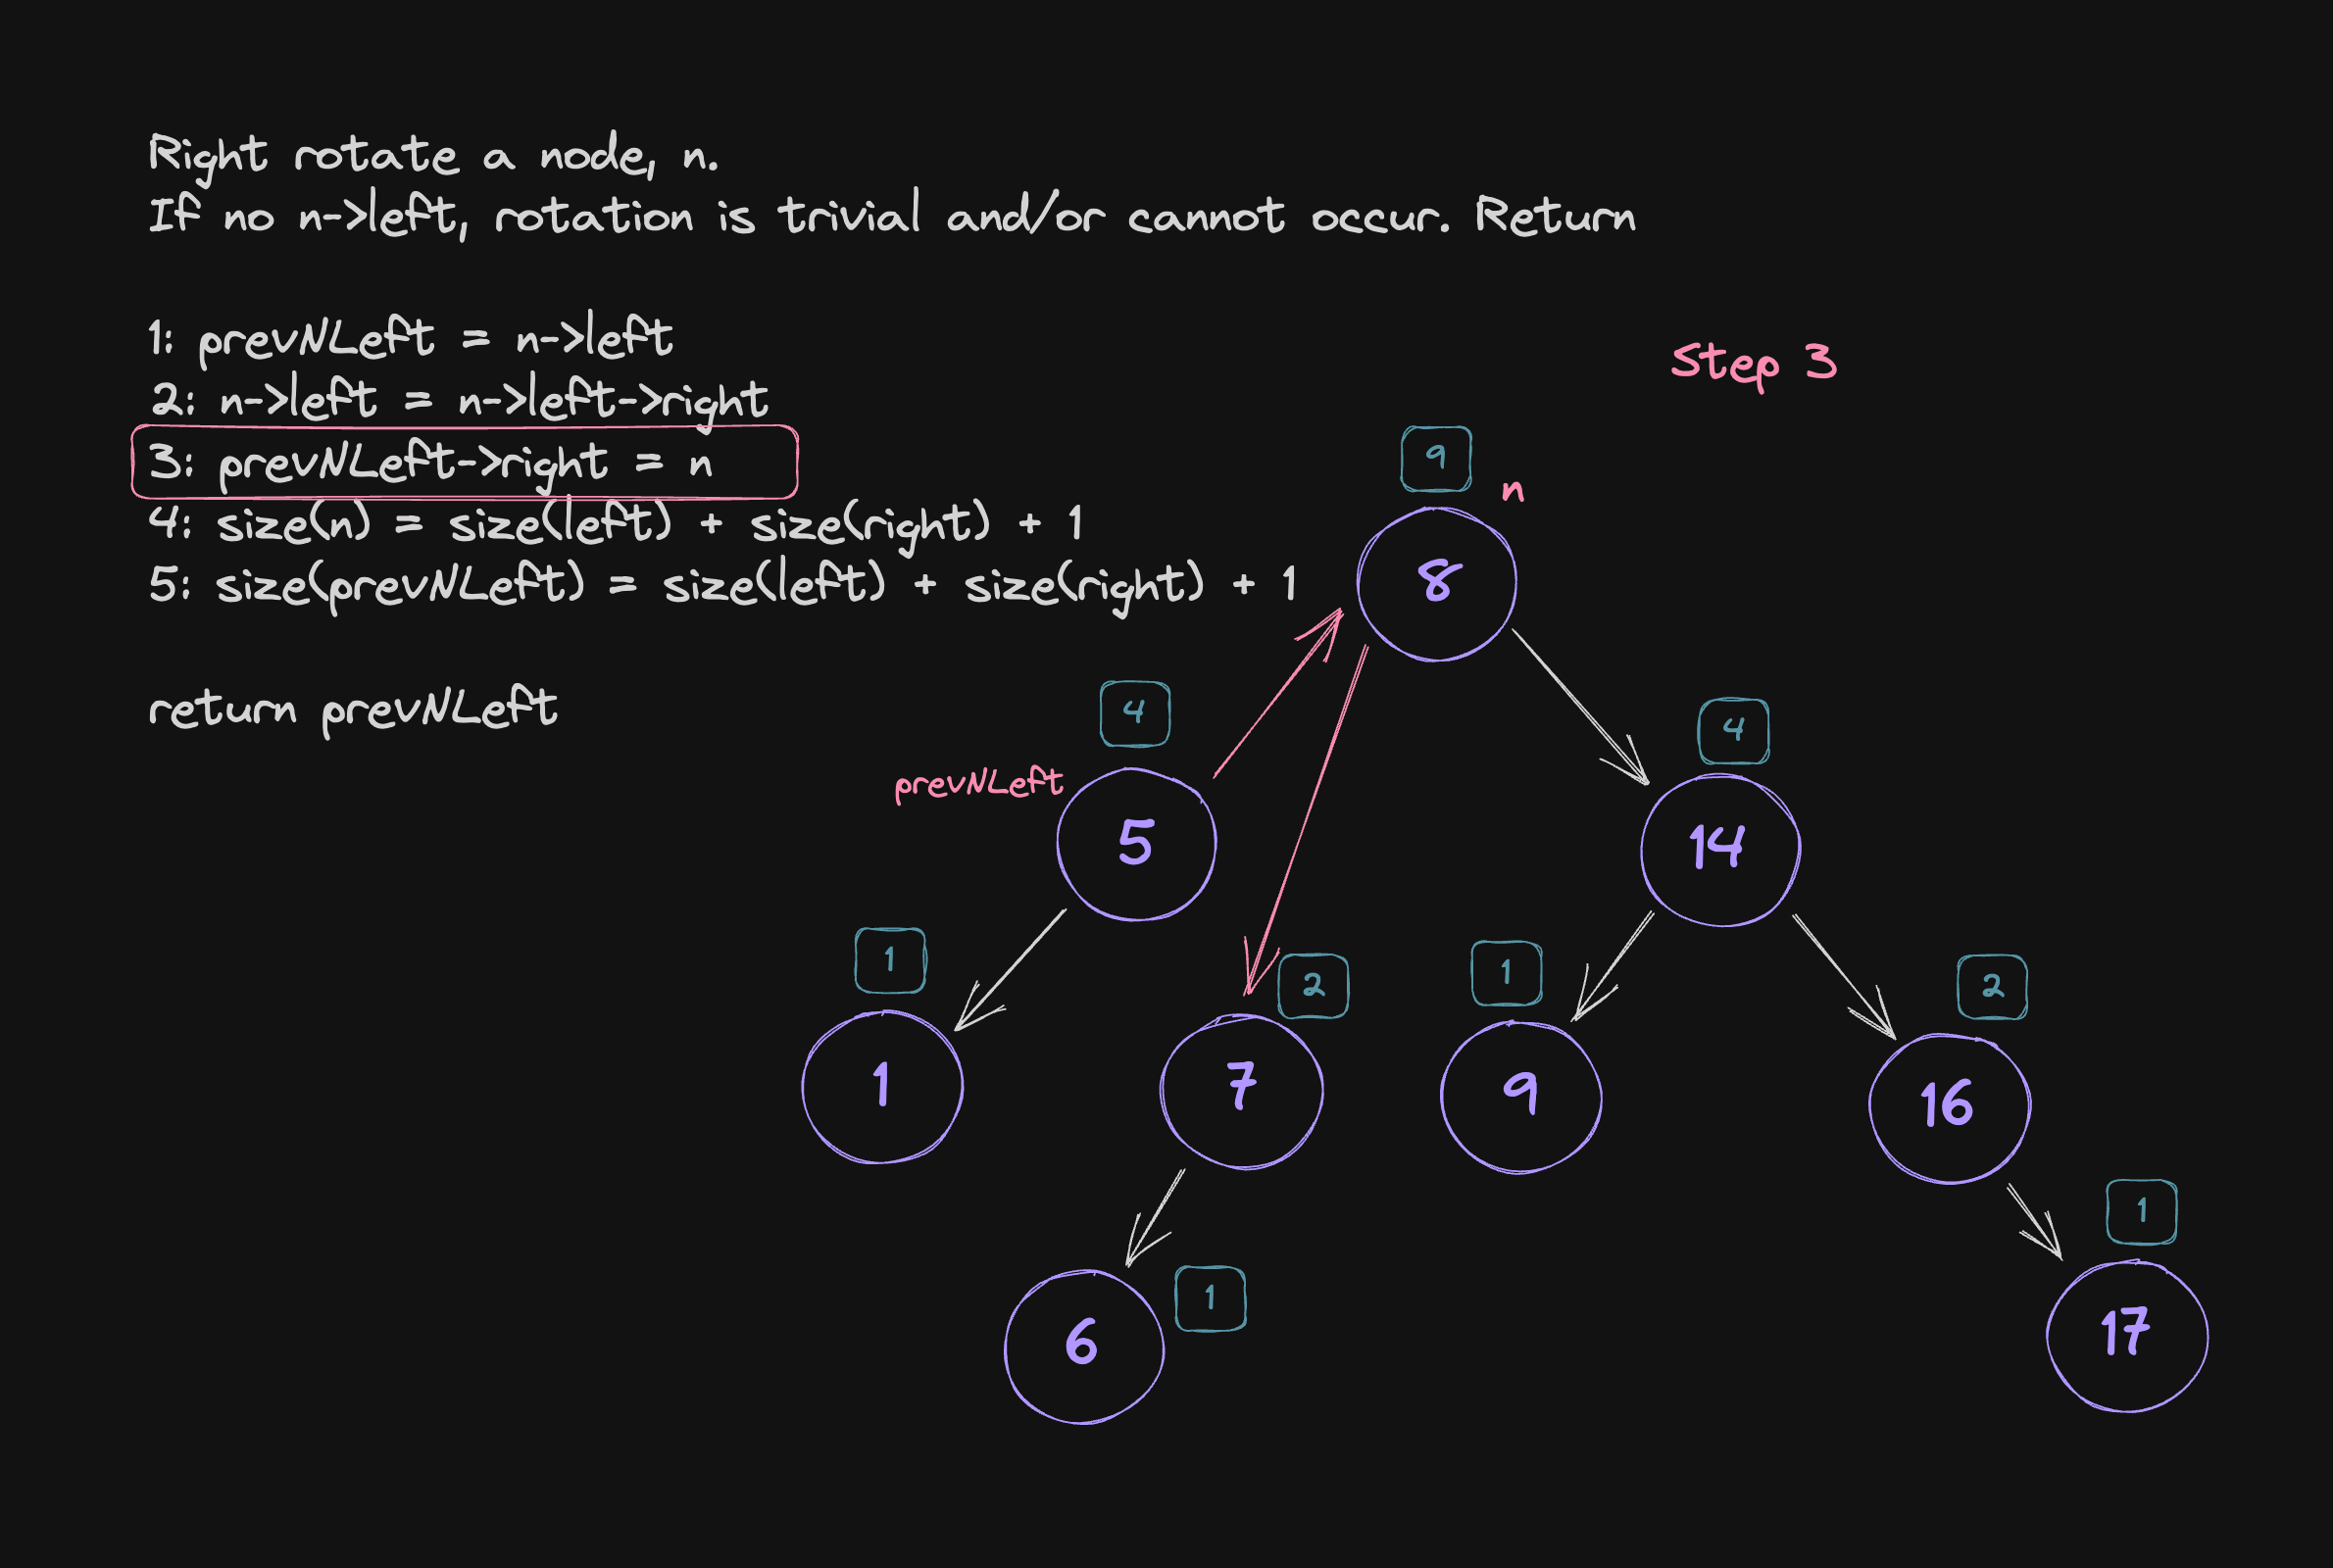
\includegraphics[scale=0.3]{right_rotations/rr3.png}         
           \newline
           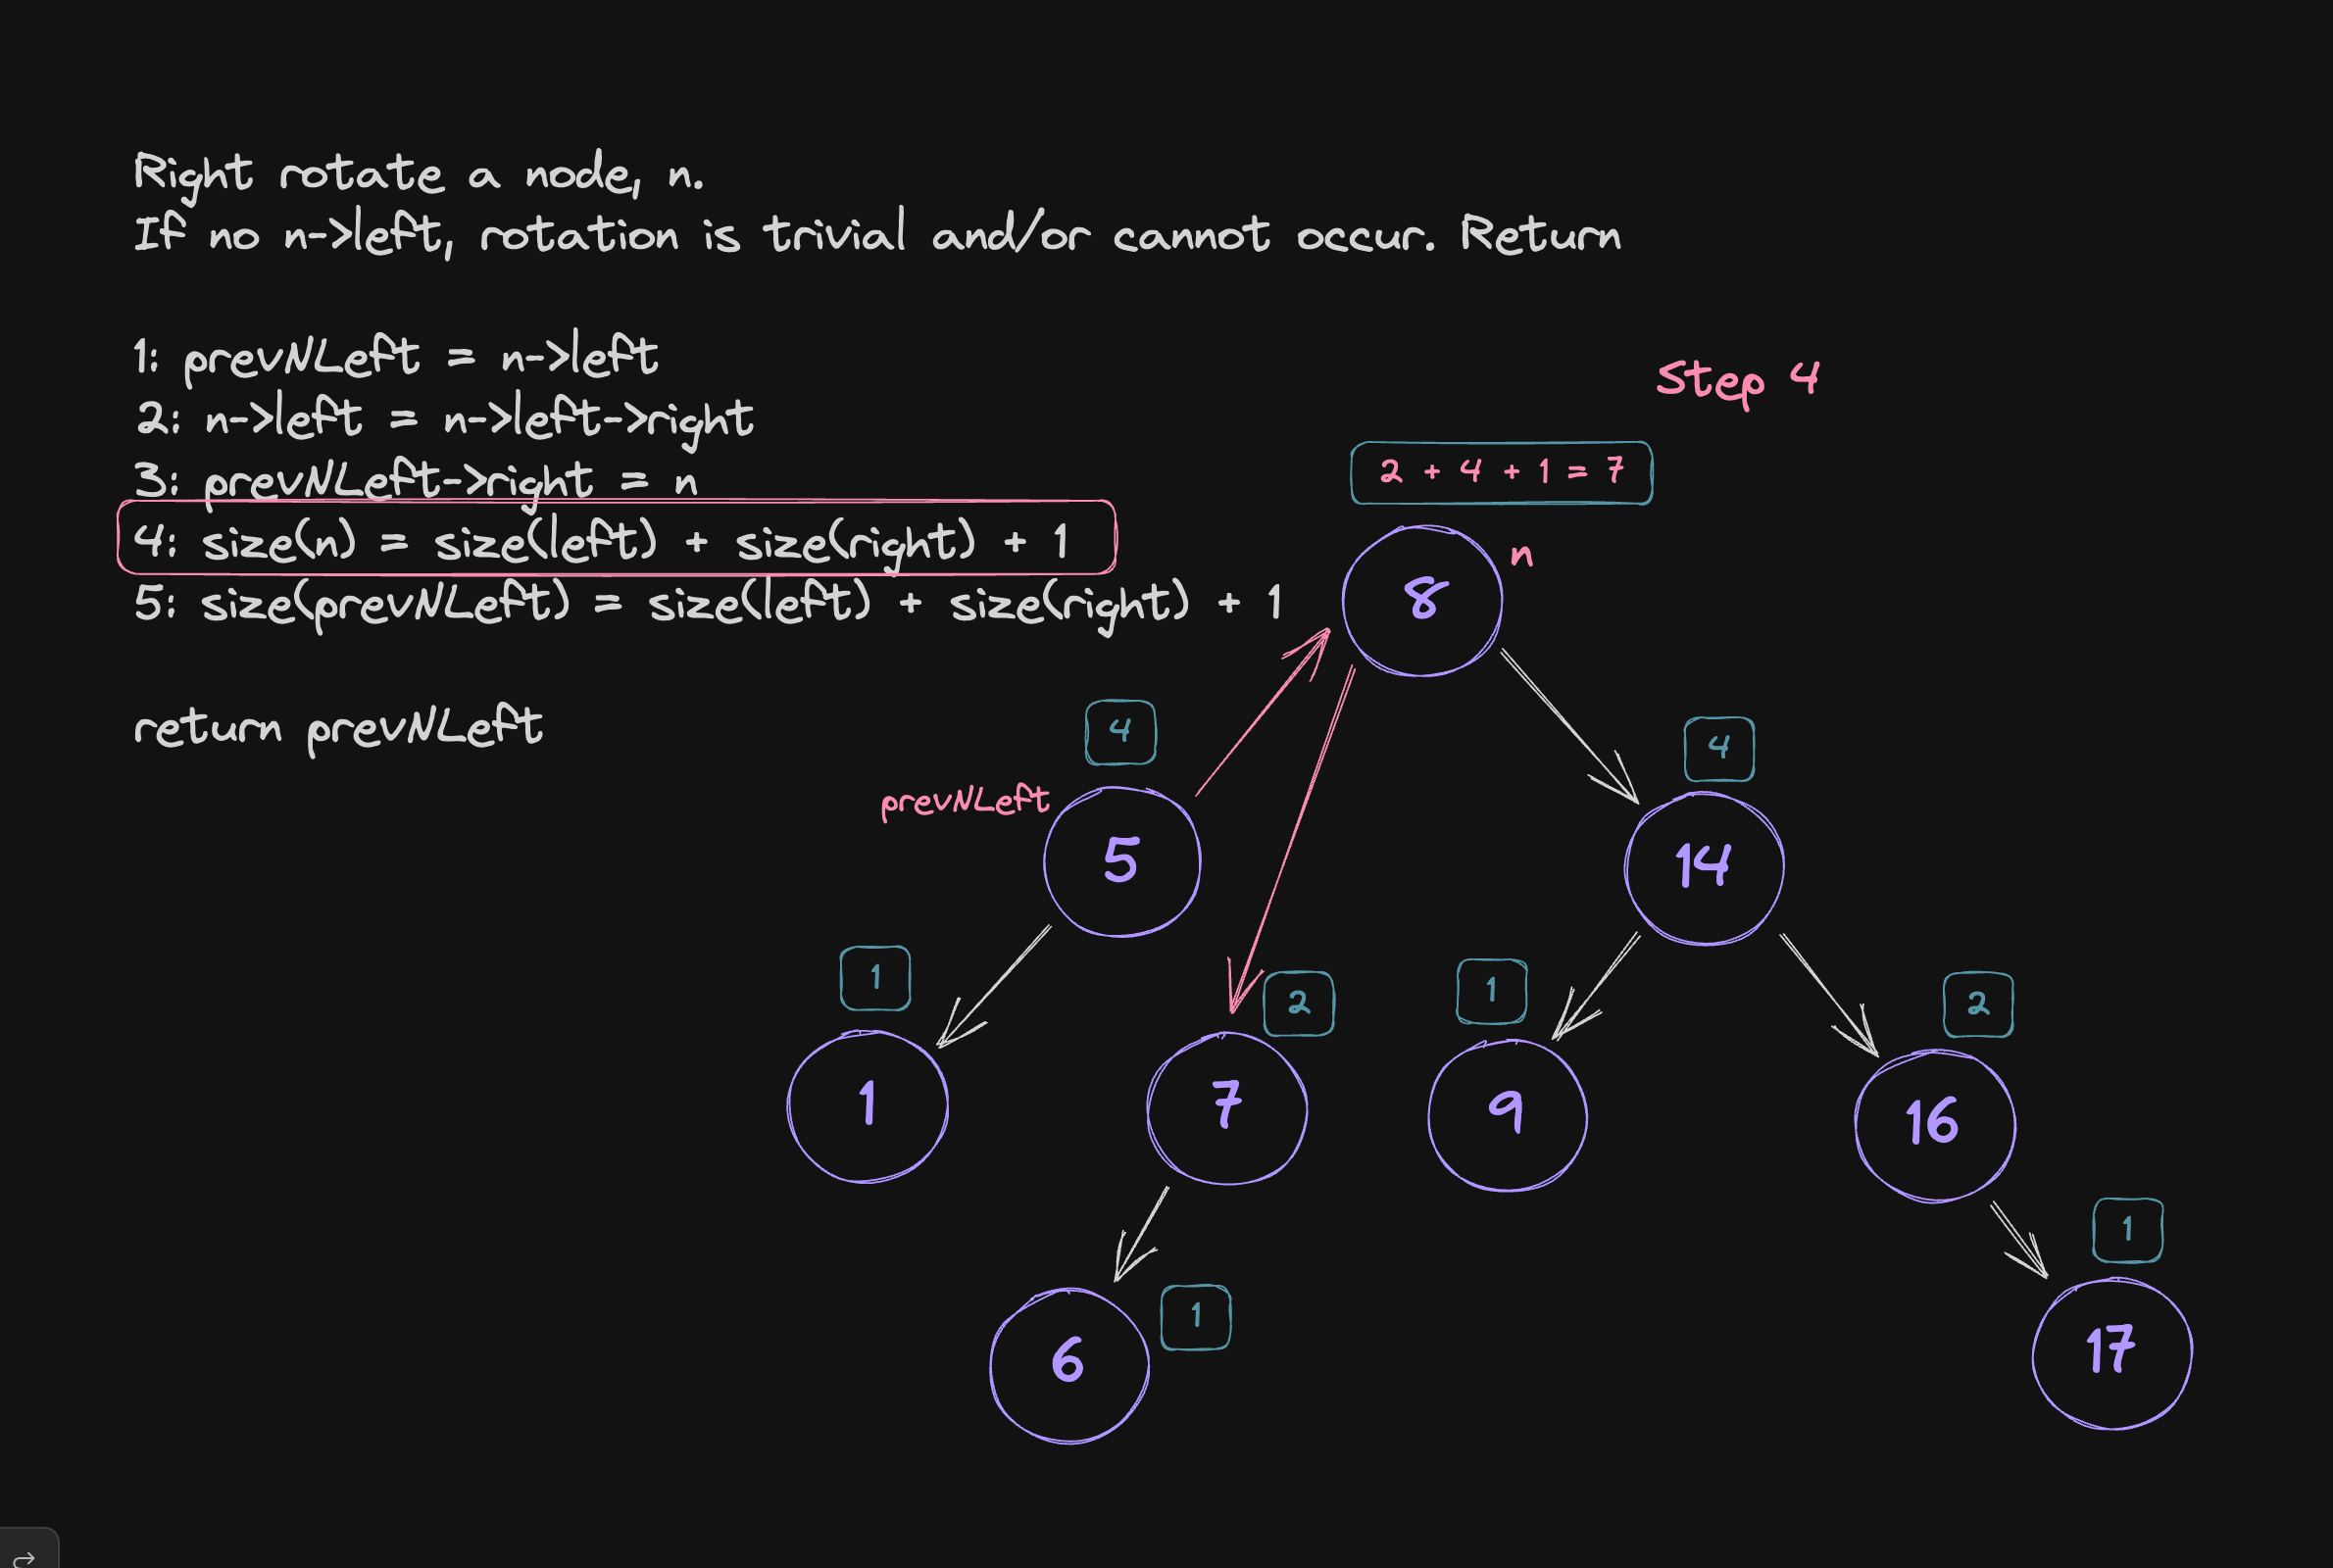
\includegraphics[scale=0.3]{right_rotations/rr4.png}         
           \newline
           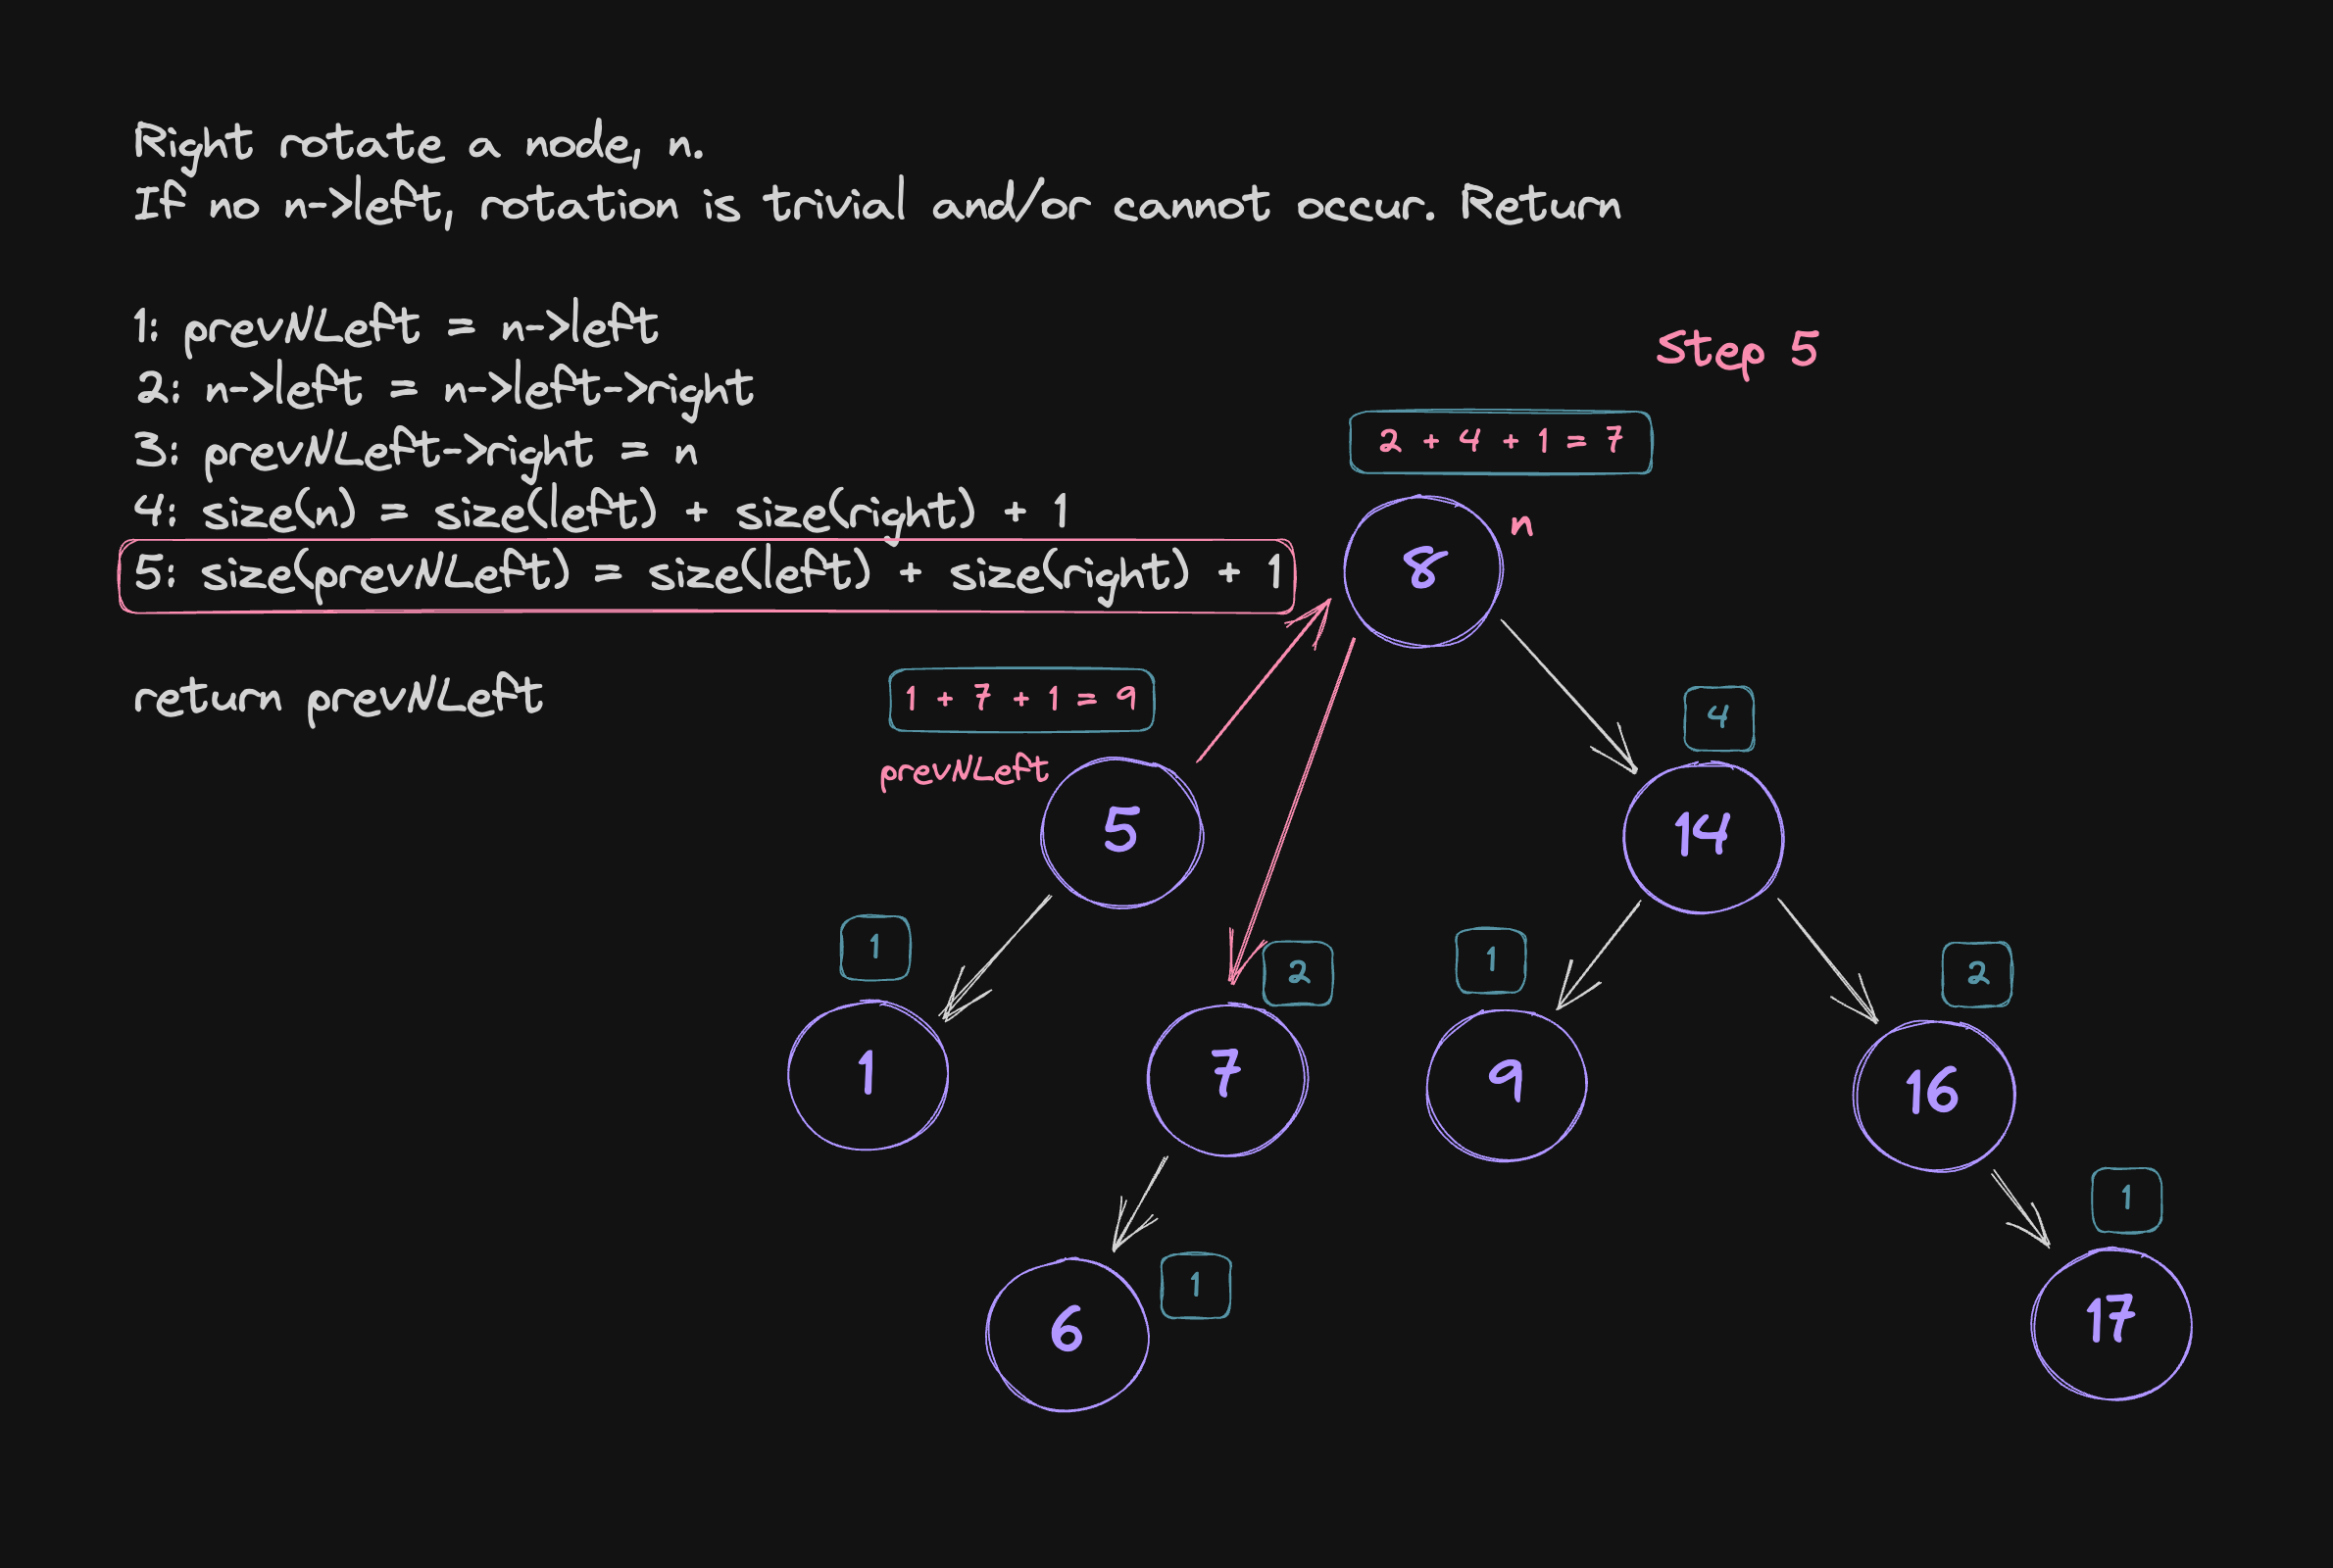
\includegraphics[scale=0.3]{right_rotations/rr5.png}         
           \newline
           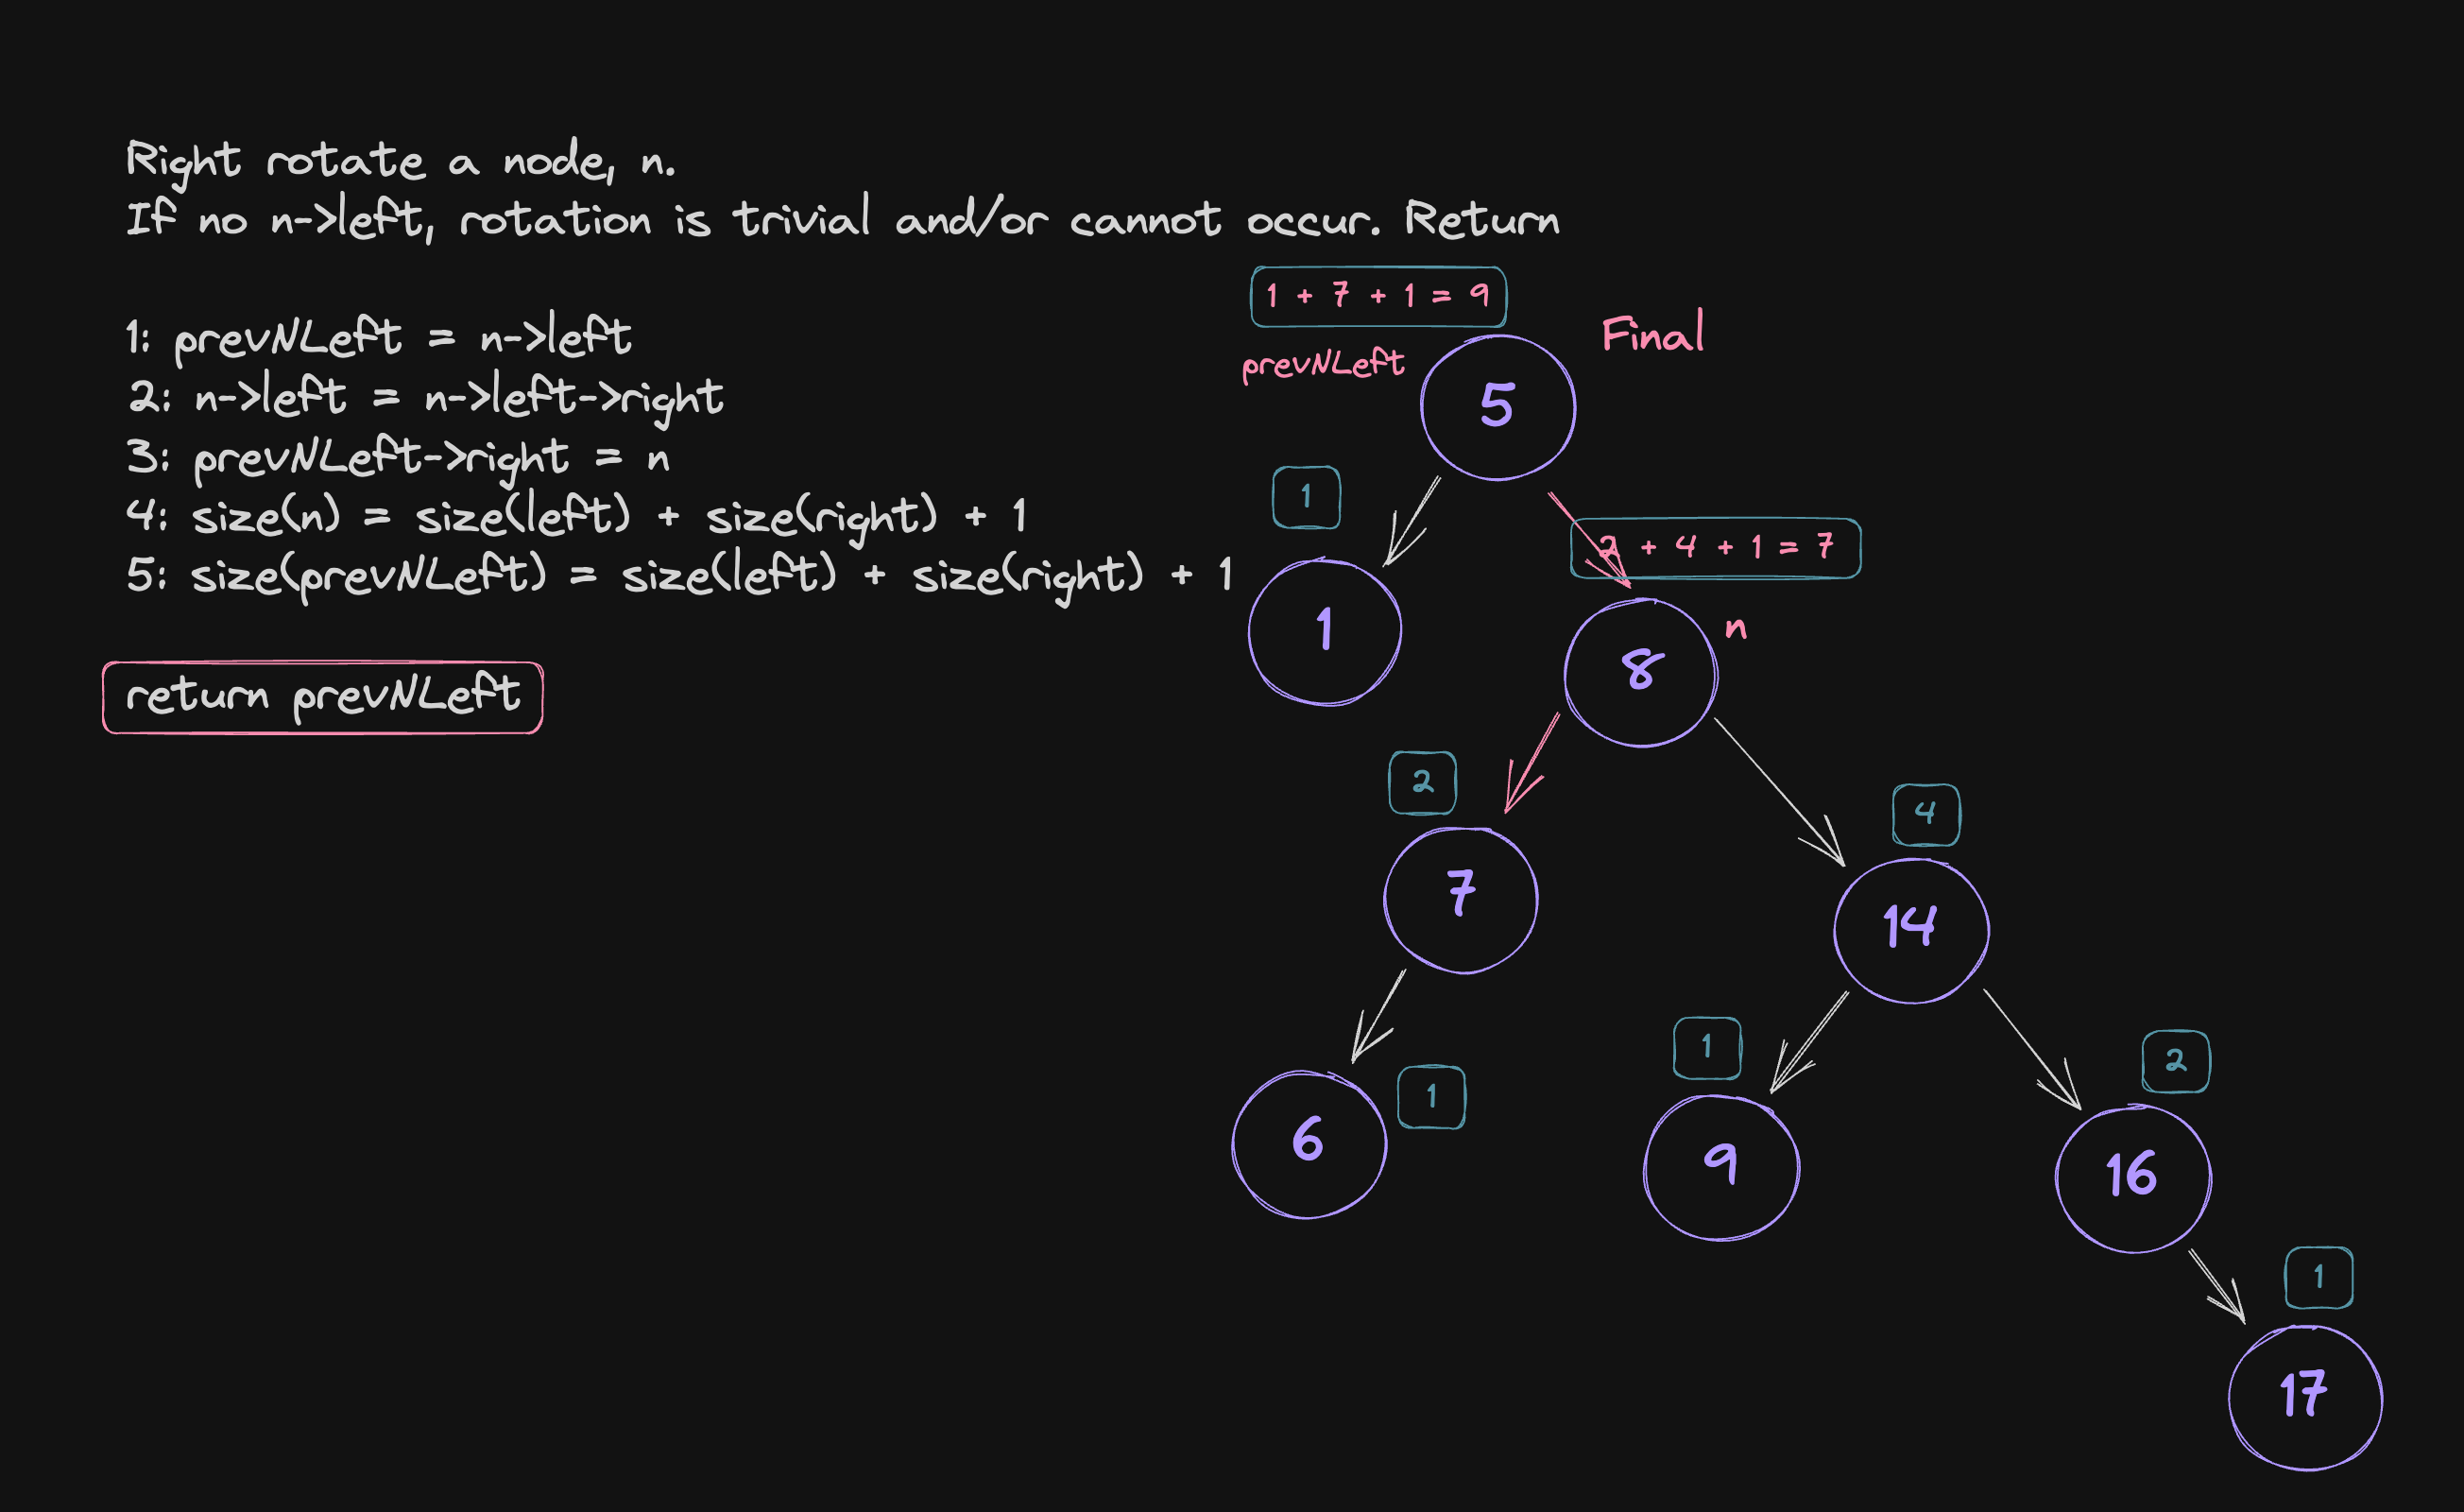
\includegraphics[scale=0.3]{right_rotations/rrf.png}         
           \newline
           \newline 
           \textbf{O(1) size updates}: \newline 
          Given a BST with correct sizes, if my right or left rotation algorithms are performed, prove the augmented tree size invariant is preserved: \newline 
          To simplify reasoning, notice that both algorithms operate on $n$, a given subtree root node, and $prevN...$, a child of $n$ where $...$ is either $Left$ or $Right$. Let $prevN$ be a substitute for either $prevNLeft$ or $prevNRight$, as the reasoning is identical. \newline 
          In both algorithms, the only nodes whose child pointers are manipulated are $n$ and $prevN$. Thus, the only modified subtrees are those rooted at $n$ and $prevN$. Assuming the input trees held correct sizing, this algorithm retains the correctness of every subtree not rooted at $n$ or $prevN$.\newline 
          After rotation, $n$ becomes a child of $prevN$. So, every left or right child tree of $n$ is an unmodified subtree. Thus, the size of $n$ can be calculated by adding the sizes of its left and right subtrees plus one for itself. An empty child tree has size zero, and a non-empty child tree already tracks its size, so this is a constant time arithmetic operation. \newline 
          The node $n$ is a child of $prevN$ in the output tree. Because one child of $prevN$ is an untouched input tree (possibly empty) and the other child is $n$, we can now assert $n$ also has a correct size and perform the same arithmetic addition as before to determine the new size of the subtree rooted at $prevN$ \newline
          After these two $O(1)$ time updates to $n$ and $prevN$ are performed, the tree's size augmentation invariant is restored.
        \end{quote}

        \newpage
        \item Implement \texttt{rotate} in size-augmented BSTs in Python in the stub we have given you.
        \begin{quote}
            \color{purple}
           \begin{minted}{python} 
    def __recalc_size(self) -> int:
        sum = 0
        if self.left:
            sum += self.left.size
        if self.right:
            sum += self.right.size
        return sum

    def __rotate_left(self) -> Self:
        prev_n_right = self.right
        assert prev_n_right is not None

        # redirect pointers
        self.right = self.right.left
        prev_n_right.left = self

        # recalculate sizes
        self.size = self.__recalc_size()
        prev_n_right.size = prev_n_right.__recalc_size()

        return prev_n_right

    def __rotate_right(self) -> Self:
        prev_n_left = self.left
        assert prev_n_left is not None

        # redirect pointers
        self.left = self.left.right
        prev_n_left.right = self

        # recalculate sizes
        self.size = self.__recalc_size()
        prev_n_left.size = prev_n_left.__recalc_size()

        return prev_n_left

    def rotate(self, direction, child_side):
        assert child_side == "L" or child_side == "R"
        assert direction == "L" or direction == "R"

        if child_side == "L":
            if direction == "L":
                self.left = self.left.__rotate_left()
            else:
                self.left = self.left.__rotate_right()
        else:
            if direction == "L":
                self.right = self.right.__rotate_left()
            else:
                self.right = self.right.__rotate_right()
        return self
           \end{minted}
        \end{quote}
        \vspace{1em}
    
    \end{enumerate}
    
    \emph{Food for thought (do read - it's an important take-away from this problem):} This problem concerns size-augmented binary search trees. In lecture, we discussed AVL trees, which are balanced binary search trees where every vertex contains an additional \textit{height} attribute containing the length of the longest path from the vertex to a leaf (height-augmented). Additionally, every pair of siblings in the tree have heights differing by at most 1, so the tree is height-balanced. Note that if we augment a binary search tree both by size (as in the above problem) and by height (and use it to maintain the AVL property), then we create a dynamic data structure able to perform \texttt{search}, \texttt{insert}, and \texttt{select} all in time $O(\log n)$. 


\end{enumerate}



\end{document}
